\documentclass{article}
%Usepackages
\usepackage{adjustbox, amsmath, amssymb, amsthm, blindtext, bm, bbm, dblfloatfix, esint, fancyhdr, float, graphicx, letltxmacro, marginnote, mathtools, subcaption, xcolor, titlesec, esint}
\usepackage{amssymb}
\usepackage[font={small, it}]{caption}
\usepackage{amsmath}
\usepackage{floatrow}
\usepackage{times}
\usepackage{ stmaryrd }
\usepackage{amsthm}
\usepackage{xcolor}
\usepackage{mathrsfs}
\usepackage[colorlinks = true,
            linkcolor = black,
            urlcolor  = blue,
            citecolor = black,
            anchorcolor = blue]{hyperref}
% \usepackage[mathscr]{euscript}
\usepackage{mathrsfs}
\usepackage{wasysym}
%\usepackage{pxfonts}
\usepackage[letterpaper, portrait, margin=1in]{geometry}
\usepackage{graphicx}
\usepackage{tikz}
\usepackage{tikz-3dplot}
\usepackage{pgfplots}
\usetikzlibrary{decorations.pathmorphing,patterns}
\usepackage{lipsum}
\usepackage{float}
\usepackage{subcaption}
\usepackage[object=vectorian]{pgfornament}
\usepackage{mwe}
\usepackage{bigints}
\usepackage{csquotes}
\usepackage{titlesec}
\usepackage{halloweenmath}
\setcounter{secnumdepth}{4}
\titleformat{\paragraph}
{\normalfont\normalsize\bfseries}{\theparagraph}{1em}{}
\titlespacing*{\paragraph}
{0pt}{3.25ex plus 1ex minus .2ex}{1.5ex plus .2ex}
\usepackage{mathtools}
\usepackage{pgfplots}
\pgfplotsset{compat=1.15}
\usepackage{lastpage}
\usepackage{enumitem}
\usepackage{tensor}
\usepackage{mathtools}

% This is for the header:
% https://tex.stackexchange.com/questions/75168/get-current-section-name-without-label
\usepackage{nameref}
\makeatletter
\newcommand*{\currentname}{\@currentlabelname}
\makeatother

\usepackage{fancyhdr} 
    \pagestyle{fancy}
    \fancyhf{}
    \fancyhead[R]{ Page \thepage \  of \pageref{LastPage}}
    \fancyhead[L]{\currentname}
\usepackage{setspace}
\usepackage{tikz}
\usetikzlibrary{hobby}

\usepackage{pst-node}
\usepackage{tikz-cd}
\usepackage[most]{tcolorbox}

% \makeatletter
% \renewcommand\@endtheorem{\vvv@endmarker\endtrivlist\@endpefalse}
% \newcommand\vvv@endmarker{%
%   {\unskip\nobreak\hfil\penalty50
%   \hskip2em\vadjust{}\nobreak\hfil\openbox
%   \parfillskip=0pt \finalhyphendemerits=0 \par
%   \penalty 10000 \parskip=0pt\noindent}\ignorespaces}
% \makeatother

\theoremstyle{definition}

% https://tex.stackexchange.com/questions/616586/how-to-make-a-tcolorbox-with-only-a-left-side-rule


\newtheorem{thm}{Theorem}[section]
\newtheorem{defn}[thm]{Definition}
\newtheorem{exmp}[thm]{Example}
\newtheorem{lem}[thm]{Lemma}
\newtheorem{conjecture}[thm]{Conjecture}
\newtheorem{exercise}[thm]{Exercise}
\newtheorem{fact}[thm]{Fact}
\newtheorem{claim}[thm]{Claim}
\newtheorem{cor}[thm]{Corollary}
\newtheorem{summary}[thm]{Summary}

\newtheorem{idea}[thm]{Idea}
\newtheorem{application}[thm]{Application}
\newtheorem{rmk}[thm]{Remark}

\newtheorem{prop}[thm]{Proposition}
\newtheorem{ques}[thm]{Question}

\newtcolorbox{cbox}[1][]{
            breakable,
            boxrule=0pt,
            frame hidden,
            sharp corners,
            enhanced,
            borderline west={2pt}{0pt}{#1},
            colback=#1!5!white}

% \newenvironment{cthm}[3]
%     {\begin{cbox}[#2]
%     \color{#2}
%     \begin{#3}[#1]
%     \color{black}
%     }
%     {
%     \end{#3} 
%     \end{cbox}
%     }

% \newenvironment{theorem}[1][]
% {\begin{cthm}{#1}{orange}{thm}}
% {\end{cthm}}

\newenvironment{theorem}[1][]
    {\begin{cbox}[blue]
    \color{blue}
    \begin{thm}[#1]
    \color{black}
    }
    {
    \end{thm} 
    \end{cbox}
    }

\newenvironment{corollary}[1][]
    {\begin{cbox}[orange]
    \color{orange}
    \begin{cor}[#1]
    \color{black}
    }
    {
    \end{cor} 
    \end{cbox}
    }

\newenvironment{lemma}[1][]
    {\begin{cbox}[orange]
    \color{orange}
    \begin{lem}[#1]
    \color{black}
    }
    {
    \end{lem} 
    \end{cbox}
    }

\newenvironment{proposition}[1][]
    {\begin{cbox}[orange]
    \color{orange}
    \begin{prop}[#1]
    \color{black}
    }
    {
    \end{prop} 
    \end{cbox}
    }

\newenvironment{definition}[1][]
    {\begin{cbox}[red]
    \color{red}
    \begin{defn}[#1]
    \color{black}
    }
    {
    \end{defn} 
    \end{cbox}
    }

\newenvironment{example}[1][]
    {\begin{cbox}[violet]
    \color{violet}
    \begin{exmp}[#1] \color{black}
    }
    {
    \end{exmp} 
    \end{cbox}
    }

\newenvironment{question}[1][]
    {\begin{cbox}[black]
    \begin{ques}[#1]
    }
    {
    \end{ques} 
    \end{cbox}
    }

\newenvironment{remark}[1][]
    {\begin{cbox}[black]
    \begin{rmk}[#1]
    }
    {
    \end{rmk} 
    \end{cbox}
    }



\newenvironment{solution}
  {\renewcommand\qedsymbol{$\blacksquare$}\begin{proof}[Solution]}
  {\end{proof}}
\newenvironment{answer}
  {\begin{proof}[Answer]}
  {\end{proof}}
  
% \newenvironment{example}
%   {\pushQED{\qed}\renewcommand{\qedsymbol}{$\triangle$}\examplex}
%   {\popQED\endexamplex}


%%%%%%%%%%%%%%%%%%%%%%%%%%%%%

%Custom Commands
    \renewcommand\qedsymbol{$\blacksquare$}
    \newcommand{\Pcal}{\mathcal{P}}
    \newcommand{\ve}{\varepsilon}
    \newcommand{\Ocal}{\mathcal{O}}
    \newcommand{\Asf}{\textsf{A}}
    \newcommand{\al}{\alpha}
    \newcommand{\be}{\beta}
    \newcommand{\Nbb}{\mathbb{N}}
    \newcommand{\Si}{\Sigma}
    \newcommand{\Hbb}{\mathbb{H}}
    \DeclareMathOperator{\diag}{diag}
    \newcommand{\De}{\Delta}
    \newcommand{\Xcal}{\mathcal{X}}
    \newcommand{\si}{\sigma}
    \newcommand{\Ga}{\Gamma}
    \newcommand{\Cscr}{\mathscr{C}}
    \newcommand{\1}{\mathbf{1}}
    \newcommand{\Dcal}{\mathcal{D}}
    \newcommand{\Iscr}{\mathscr{I}}
    \newcommand{\Pbb}{\mathbb{P}}
    \newcommand{\B}{\mathbb{B}}
    \newcommand{\Dscr}{\mathscr{D}}
    \newcommand{\Nfrak}{\mathfrak{N}}
    \newcommand{\Efrak}{\mathfrak{E}}
    \DeclareMathOperator{\charp}{charpoly}
    \newcommand{\Csf}{\mathsf{C}}
    \newcommand{\rfrak}{\mathfrak{r}}
    \newcommand{\Sbb}{\mathbb{S}}
    \newcommand{\La}{\Lambda}
    \newcommand{\de}{\delta}
    \DeclareMathOperator{\inte}{int}
    \DeclareMathOperator{\ord}{ord}
    \newcommand{\set}{\mathsf{set}}
    \newcommand{\Bscr}{\mathscr{B}}
    \newcommand{\Zscr}{\mathscr{Z}}
    \newcommand{\ab}{\mathrm{ab}}
    \newcommand{\Xscr}{\mathscr{X}}
    \newcommand{\Escr}{\mathscr{E}}
    \newcommand{\Gscr}{\mathscr{G}}
    \DeclareMathOperator{\Sym}{Sym}
    \newcommand{\om}{\omega}
    \newcommand{\gfrak}{\mathfrak{g}}
    \newcommand{\hfrak}{\mathfrak{h}}
    \newcommand{\kfrak}{\mathfrak{k}}
    \newcommand{\Grp}{\mathsf{Grp}}
    \newcommand{\Ab}{\mathsf{Ab}}
    \newcommand{\xbar}{\bar{x}}
    \newcommand{\abar}{\bar{a}}
    \newcommand{\ybar}{\bar{y}}
    \DeclareMathOperator{\coker}{coker}
    \newcommand{\Modsf}{\mathsf{Mod}}
    \newcommand{\op}{\mathrm{op}}
    \newcommand{\Ring}{\mathsf{Ring}}
    \newcommand{\modsf}{\mathsf{mod}}
    \DeclareMathOperator{\Alt}{Alt}
    \newcommand{\Om}{\Omega}
    \newcommand{\ze}{\zeta}
    \newcommand{\Fcal}{\mathcal{F}}
    \newcommand{\Oscr}{\mathscr{O}}
    \newcommand{\gl}{\mathfrak{gl}}
    \DeclareMathOperator{\Lie}{Lie}
    \DeclareMathOperator{\GL}{GL}
    \DeclareMathOperator{\SL}{SL}
    \DeclareMathOperator{\Vol}{Vol}
    \DeclareMathOperator{\Disc}{Disc}
    \DeclareMathOperator{\SO}{SO}
    \newcommand{\Xfrak}{\mathfrak{X}}
    \DeclareMathOperator{\id}{id}
    \DeclareMathOperator{\Int}{Int}
    \DeclareMathOperator{\End}{End}
    \DeclareMathOperator{\Aut}{Aut}
    \DeclareMathOperator{\stab}{stab}
    \DeclareMathOperator{\orb}{orb}
    \DeclareMathOperator{\grad}{grad}
    \DeclareMathOperator{\curl}{curl}
    \newcommand{\vp}{\varphi}
    \newcommand{\vt}{\vartheta}
    \DeclareMathOperator{\Gal}{Gal}
    \DeclareMathOperator{\rank}{rank}
    \DeclareMathOperator{\col}{col}
    \DeclareMathOperator{\Tame}{Tame}  
    \newcommand{\Yscr}{\mathscr{Y}}
    \newcommand{\Fbb}{\mathbb{F}}
    \newcommand{\Hcal}{\mathcal{H}}
    \newcommand{\arctanh}{\text{arctanh}}
    \newcommand{\pa}{\partial}
    \newcommand{\del}{\boldsymbol{\nabla}}
    \newcommand{\na}{\nabla}
    \newcommand{\Ycal}{\mathcal{Y}}
    \DeclareMathOperator{\spn}{span}
    \DeclareMathOperator{\Inn}{Inn}
    \DeclareMathOperator{\Proj}{Proj}
    \DeclareMathOperator{\chara}{char}
    \newcommand{\lap}{\nabla^2}
    \newcommand{\Pfrak}{\mathfrak{P}}
    \newcommand{\mfrak}{\mathfrak{m}}
    \newcommand{\Fvec}{\mathbf{F}}
    \newcommand{\Mcal}{\mathcal{M}}
    \newcommand{\ellvec}{\boldsymbol{\ell}}
    \newcommand{\rvec}{\mathbf{r}}
    \DeclareMathOperator{\supp}{supp}
    \newcommand{\Abb}{\mathbb{A}}
    \newcommand{\svec}{\mathbf{s}}
    \newcommand{\VECT}{\mathsf{VECT}}
    \newcommand{\fs}{\vec{\sigma}}
    \newcommand{\bs}{\cev{\sigma}}
    \newcommand{\uvec}{\mathbf{u}}
    \newcommand{\iunit}{\boldsymbol{\hat{\i}}}
    \newcommand{\junit}{\boldsymbol{\hat{\j}}}
    \newcommand{\xunit}{\mathbf{\hat{x}}}
    \newcommand{\Char}{\text{char}}
    \newcommand{\kunit}{\mathbf{\hat{k}}}
    \newcommand{\theunit}{\boldsymbol{\hat{\theta}}}
    \newcommand{\pvec}{\mathbf{p}}
    \newcommand{\qvec}{\mathbf{q}}
    \newcommand{\Qcal}{\mathcal{Q}}
    \newcommand{\yvec}{\mathbf{y}}
    \newcommand{\xvec}{\mathbf{x}}
    \newcommand{\wvec}{\mathbf{w}}
    \newcommand{\bvec}{\mathbf{b}}
    \newcommand{\Ucal}{\mathcal{U}}
    \newcommand{\Ncal}{\mathcal{N}}
    \newcommand{\Scal}{\mathcal{S}}
    \newcommand{\Nscr}{\mathscr{N}}
    \newcommand{\da}{\dagger}
    \newcommand{\CT}{\mathrm{H}}
    \newcommand{\Sscr}{\mathscr{S}}
    \DeclareMathOperator{\lcm}{lcm}
    \newcommand{\evec}{\mathbf{e}}
    \newcommand{\Kscr}{\mathscr{K}}
    \newcommand{\ebold}{\boldsymbol{e}}
    \newcommand{\zvec}{\mathbf{z}}
    \newcommand{\vvec}{\mathbf{v}}
    \newcommand{\Tscr}{\mathscr{T}}
    \newcommand{\avec}{\mathbf{a}}
    \newcommand{\Avec}{\mathbf{A}}
    \newcommand{\Ivec}{\mathbf{I}}
    \newcommand{\ivec}{\mathbf{i}}
    \newcommand{\jvec}{\mathbf{j}}
    \newcommand{\kvec}{\mathbf{k}}
    \newcommand{\of}{\mathfrak{o}}
    \DeclareMathOperator{\Ot}{O}
    \DeclareMathOperator{\Sy}{S}
    \newcommand{\slf}{\mathfrak{sl}}
    \newcommand{\muvec}{\boldsymbol{\mu}}
    \newcommand{\Bvec}{\mathbf{B}}
    \newcommand{\Cvec}{\mathbf{C}}
    \newcommand{\eunit}{\mathbf{\hat{e}}}
    \newcommand{\vpunit}{\boldsymbol{\hat{\varphi}}}
    \newcommand{\zero}{\boldsymbol{0}}
    \newcommand{\tauvec}{\boldsymbol{\tau}}
    \newcommand{\runit}{\mathbf{\hat{r}}}
    \newcommand{\U}{\mathcal{U}}
    \newcommand{\Zbb}{\mathbb{Z}}
    \newcommand{\Bsf}{\mathsf{B}}
    \DeclareMathOperator{\G}{G}
    \newcommand{\gmat}{\textsf{g}}
    \newcommand{\Ccal}{\mathcal{C}}
    \newcommand{\SM}{\mathsf{SM}}
    \newcommand{\VB}{\mathsf{VB}}
    \newcommand{\Dsf}{\mathsf{D}}
    \newcommand{\Fscr}{\mathscr{F}}
    \DeclareMathOperator{\Map}{Map}
    \DeclareMathOperator{\Frob}{Frob}
    \newcommand{\Imat}{\textsf{I}}
    \newcommand{\Rmat}{\textsf{R}}
    \DeclareMathOperator{\Frac}{Frac}
    \DeclareMathOperator{\Spec}{Spec}
    \DeclareMathOperator{\Emb}{Emb}
    \newcommand{\Kcal}{\mathcal{K}}
    \newcommand{\Wcal}{\mathcal{W}}
    \newcommand{\Lcal}{\mathcal{L}}
    \newcommand{\Tcal}{\mathcal{T}}
    \newcommand{\Ecal}{\mathcal{E}}
    \DeclareMathOperator{\im}{im}
    \newcommand{\Qbb}{\mathbb{Q}}
    \newcommand{\ga}{\gamma}
    \newcommand{\la}{\lambda}
    \newcommand{\RomanNumeralCaps}[1]
        {\MakeUppercase{\romannumeral #1}} 
    \newcommand{\dif}{\text{d}}
    \newcommand{\Rbb}{\mathbb{R}}
    \newcommand{\Tbb}{\mathbb{T}}
    \DeclareMathOperator{\Hom}{Hom}
    \DeclareMathOperator{\conv}{conv}
    \newcommand{\Vcat}{\mathsf{V}}
    \newcommand{\Gr}{\text{Gr}}
    \newcommand{\Bcal}{\mathcal{B}}
    \newcommand{\Acal}{\mathcal{A}}
    \newcommand{\pfrak}{\mathfrak{p}}
    \newcommand{\qfrak}{\mathfrak{q}}
    \newcommand{\Evec}{\mathbf{E}}
    \newcommand{\omvec}{\boldsymbol{\omega}}
    \newcommand{\alvec}{\boldsymbol{\alpha}}
    \newcommand{\gvec}{\mathbf{g}}
    \newcommand{\afrak}{\mathfrak{a}}
    \newcommand{\bfrak}{\mathfrak{b}}
    \newcommand{\Cbb}{\mathbb{C}}
    \newcommand{\gavec}{\boldsymbol{\gamma}}
    \newcommand{\Tvec}{\mathbf{T}}
    \newcommand{\Vscr}{\mathscr{V}}
    \newcommand{\Ascr}{\mathscr{A}}
    \newcommand{\Uscr}{\mathscr{U}}
    \newcommand{\Sfrak}{\mathfrak{S}}
    \DeclareMathOperator{\sgn}{sgn}
    \DeclareMathOperator{\vol}{vol}
    \newcommand{\Pscr}{\mathscr{P}}
    \newcommand{\Wscr}{\mathscr{W}}
    \newcommand{\bcdot}{\boldsymbol{\cdot}}
    \DeclareMathOperator{\tr}{tr}
    
    \newcommand{\sectionline}{
        \noindent
        \begin{center}
        {
        {{
        {\begin{tikzpicture}
        \node  (C) at (0,0) {};
        \node (D) at (16,0) {};
        \path (C) to [ornament=89] (D);
        \end{tikzpicture}}}}}
        \end{center}
        }
    \newcommand{\sectionlineflip}{
        \noindent
        \begin{center}
        {
        {{
        {\begin{tikzpicture}
        \node  (C) at (0,0) {};
        \node (D) at (16,0) {};
        \path (D) to [ornament=89] (C);
        \end{tikzpicture}}}}} 
        \end{center}
        }
        

        
       
%%%%%%%%%%%%%%%%%%%%%%%%%%%%%%%
%Custom Symbols
\newcommand{\goodemptyset}[1]{%
\begin{tikzpicture}[#1]%
\draw (0,0) circle (0.1);%
\draw(-0.07,-0.14)--(0.07,0.14);
\end{tikzpicture}%
}

\newcommand{\es}{\raisebox{-1pt}{\goodemptyset{}}}


\makeatletter
\DeclareRobustCommand{\cev}[1]{%
  {\mathpalette\do@cev{#1}}%
}
\newcommand{\do@cev}[2]{%
  \vbox{\offinterlineskip
    \sbox\z@{$\m@th#1 x$}%
    \ialign{##\cr
      \hidewidth\reflectbox{$\m@th#1\vec{}\mkern4mu$}\hidewidth\cr
      \noalign{\kern-\ht\z@}
      $\m@th#1#2$\cr
    }%
  }%
}
\makeatother


\makeatletter
\DeclarePairedDelimiterX{\pmodx}[1]{(}{)}{{\operator@font mod}\mkern6mu#1}
\renewcommand{\pmod}{%
  \allowbreak
  \if@display\mkern18mu\else\mkern8mu\fi
  \pmodx
}
\makeatother
\DeclarePairedDelimiter\bra{\langle}{\rvert}
\DeclarePairedDelimiter\ket{\lvert}{\rangle}
\DeclarePairedDelimiterX\braket[2]{\langle}{\rangle}{#1 \delimsize\vert #2}

 
\makeatletter
\newcommand{\colim@}[2]{%
  \vtop{\m@th\ialign{##\cr
    \hfil$#1\operator@font colim$\hfil\cr
    \noalign{\nointerlineskip\kern1.5\ex@}#2\cr
    \noalign{\nointerlineskip\kern-\ex@}\cr}}%
}
\newcommand{\colim}{%
  \mathop{\mathpalette\colim@{\rightarrowfill@\scriptscriptstyle}}\nmlimits@
}
\renewcommand{\varinjlim}{%
  \mathop{\mathpalette\varlim@{\rightarrowfill@\scriptscriptstyle}}\nmlimits@
}
\renewcommand{\varprojlim}{%
  \mathop{\mathpalette\varlim@{\leftarrowfill@\scriptscriptstyle}}\nmlimits@
}

\newcommand{\mjedit}[1]{{\color{orange}  #1}}
\newcommand{\mattie}[1]{{\color{orange} \sf $\clubsuit\clubsuit\clubsuit$ Mattie: [#1]}}
\newcommand{\margMa}[1]{\normalsize{{\color{red}\footnote{{\color{orange}#1}}}{\marginpar[{\color{red}\hfill\tiny\thefootnote$\rightarrow$}]{{\color{red}$\leftarrow$\tiny\thefootnote}}}}}
\newcommand{\Mattie}[1]{\margMa{(Mattie) #1}}


% %%%%%%%%%%%%%%%%%%%%%%%%%%%%%
% %Just arrows (cause normy arrows suck)
% \newcommand{\goodarrow}[1]{
% \begin{tikzpicture}[#1]
% \draw[-stealth] (0,0)--(0.4,0);
% \end{tikzpicture}
% }

% \renewcommand{\to}{\raisebox{2.4pt}{\hspace{0.08cm}\goodarrow{}\hspace{0.06cm}}}

% %%%%

% \newcommand{\goodtwoheadrightarrow}[1]{
% \begin{tikzpicture}[#1]
% \draw[->>, >=stealth] (0,0)--(0.4,0);
% \end{tikzpicture}
% }

% \renewcommand{\twoheadrightarrow}{\raisebox{2.4pt}{\hspace{0.08cm}\goodtwoheadrightarrow{}\hspace{0.06cm}}}

% %%%

% \newcommand{\goodhookrightarrow}[1]{
% \begin{tikzpicture}[#1]
% \draw[right hook-stealth] (0,0)--(0.4,0);
% \end{tikzpicture}
% }

% \renewcommand{\hookrightarrow}{\raisebox{2.3pt}{\hspace{0.08cm}\goodhookrightarrow{}\hspace{0.06cm}}}

% %%%

% \newcommand{\goodmapsto}[1]{
% \begin{tikzpicture}[#1]
% \draw[-stealth] (0,0)--(0.4,0);
% \draw[] (0,0.06)--(0,-0.06);
% \end{tikzpicture}
% }

% \renewcommand{\mapsto}{\raisebox{0pt}{\hspace{0.02cm}\goodmapsto{}\hspace{0.03cm}}}


% %%%%%%%%%%%%%%%%%%%%%%%%%%%%%

% \tikzcdset{arrow style=tikz, diagrams={>={stealth[round,length=4pt,width=4.5pt,inset=2.75pt]}}}






\renewcommand*\contentsname{Table of Content}

\title{MATH 2260 Spring 2024 Notes}
\author{Mattie Ji}
\date{Updated \today}
\setlength\parindent{0pt}

\begin{document}

\maketitle
These are lecture notes from \textbf{MATH 2060: Complex Function Theory II - Riemann Surfaces} with Professor Jeremy Kahn at Brown University for the Spring 2024 semester.\\

These notes are taken by Mattie Ji with gracious help and input from the instructor of this course. If you find any mistakes in these notes, please feel free to direct them via email to me or send a pull request on GitHub.\\
\tableofcontents

\newpage

 
\newpage
\section{Lecture January 25th}

\textbf{Instructor: Jeremy Kahn}

\subsection{Syllabus}

Despite being called ``Complex Function Theory II", this is a course on Riemann Surfaces (RS). This course is divided into three parts:
\begin{enumerate}
    \item Definitions and Constructions of Riemann Surfaces.
    \item Compact Riemann Surfaces, where we will prove the usual theorems
    \begin{itemize}
        \item Mittag-Leffler, Riemann-Roch, Abel and Jacobi.
        \item Functions and forms on Compact Riemann Surfaces.
        \item Solving $\overline{\partial} f = \alpha$ (the ``d-bar equation").
    \end{itemize}
    \item Uniformization and Hyperbolic Geometry. The uniformization theorem that classifies all simply connected Riemann surfaces (it turns out that most of them are quotients of the hyperbolic plane.) We will also talk about closed geodesics and cusps. We will also talk about Pants decomposition and Mumford's theorem.
\end{enumerate}
One thing we will not do is \textbf{sheaves and sheaf cohomology}. This is because these theorems can all be done without the language of sheaves.\\

\textbf{Interaction and Feedback:}
\begin{itemize}
    \item Class participation is strongly encouraged.
    \item There's traditionally a recitation where someone presents the solution to a problem.
    \item There aren't exactly homeworks, but there are weekly opportunities to turn in one or two solutions you are especially proud of.
    \item There might be an optional presentation at the end.
\end{itemize}

\textbf{Textbook: } In principle, the primary textbook should be the notes (still under some constructions) sent out by the instructor. There are also supplementary references. The main one is Forster, which the course is \textbf{loosely} adapted from.\\

\textbf{Office Hours: } Thursday 4 - 5 pm right after class, or by appointment.\\

\textbf{Pre-requisites:}
\begin{itemize}
    \item In principle, it should just be Complex Function Theory I. However, ...
    \item Fundamental groups and covering spaces.
    \item Singular homology and cohomology. De Rham Cohomology.
    \item Point-set topology.
\end{itemize}

\subsection{Introduction}

\begin{definition}
    A Riemann surface is a topological space $X$ along with a set $\{(U_\alpha, \phi_\alpha: U_\alpha \to \Cbb)\}$ of \textbf{charts} such that
    \begin{enumerate}
        \item $X$ is Hausdorff.
        \item For all $\alpha$; $U_\alpha \subset X$ is open, $\varphi_\alpha: U_\alpha \to \Cbb$ is an embedding, and $\varphi_\alpha(U_\alpha)$ is open in $\Cbb$ (note that we are not requiring the image to be simply connected).
        \item The union over all $\alpha$ of $U_\alpha$ is $X$, ie. $\bigcup_{\alpha} U_\alpha = X$.
        \item $\phi_\alpha \circ \phi_\beta^{-1}: \varphi_\beta(U_\alpha \cap U_\beta) \to \varphi_\alpha(U_\alpha \cap U_\beta)$ is holomorphic.
        \item $X$ is second countable.
        \item $X$ is connected.
    \end{enumerate}
    Note that if the last condition is removed, then $X$ is the definition of a complex $1$-manifold. For Riemann Surfaces, we only care about connected ones.
\end{definition}

\begin{remark}
    The condition that $X$ being second countable is actually implied by the other conditions listed here, but this is a very deep theorem.
\end{remark}

\begin{example}
    Here are some examples of Riemann surfaces.
    \begin{enumerate}
        \item Let $U \subseteq \Cbb$ be an open subset of $\Cbb$, then $U$ is a Riremann surface with a global chart.
        \item Let $X = \Hat{\Cbb} = \Cbb \cup \{\infty\}$ be the Riemann sphere. Then consider $U_0 = \Cbb$ and $U_1 = (\Cbb \setminus \{0\}) \cup \{\infty\}$. Let $\varphi_0$ be the identity and $\varphi_1(z) = \frac{1}{z}$. In this case, $\varphi_0(U_0) = \Cbb$ and $\varphi_1(U_1) = \Cbb$. The transition map is holomorphic because it is just $1/z$ on $\Cbb \setminus \{0\}$.
        \item Here's a motivational picture of a Riemann surface:
        \[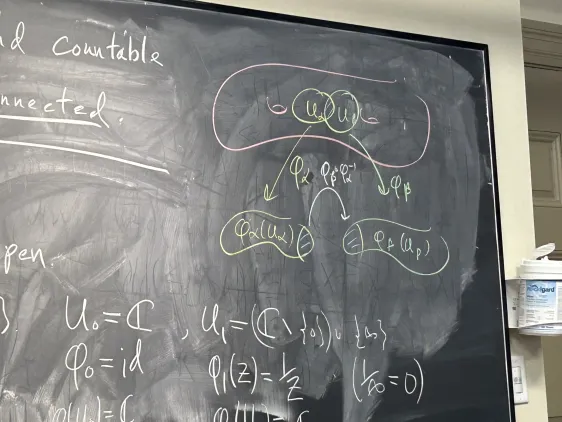
\includegraphics[width=0.5\textwidth]{Figures/cft-1.png}.\]
    \end{enumerate}
\end{example}

\begin{definition}
    A continuous map $f: X \to Y$ with $X, Y$ being Riemann surfaces is \textbf{holomorphic} if for all $\varphi: U \to \Cbb$ and $\psi: V \to \Cbb$ charts on $X$ and $Y$ respectively, then 
    \[\psi \circ f \circ \varphi^{-1} \text{ is holomorphic on $\varphi(f^{-1}(V) \cap U)$}.\]
\end{definition}

\begin{theorem}[Theorem]
    Let $f: X \to Y$ and $g: Y \to Z$ where $X, Y, Z$ Riemann surfaces. Then
    \[f, g \text{ is holomorphic } \implies g \circ f \text{ is holomorphic}.\]
    $f$ is a biholomorphism if $f$ is furthermore bijective and $f^{-1}$ is holomorphic.
\end{theorem}


\begin{example}[Different Choices of Charts can lead to different structures]
Note that different choices of charts on the same topological space $X$ could lead to different Riemann surfaces.\\

Take $\mathbb{D} \subseteq \Cbb$. Consider two different charts $\varphi: \mathbb{D} \to \Cbb$ by $\varphi(z) = z$ and $\psi: \mathbb{D} \to \Cbb, \psi(r e^{i\theta}) =  \frac{r}{1-r} e^{i\theta}$ (where we are taking the disk to the entire complex plane essentially). Certainly there are no biholomorphism between the two, otherwise it would imply that there's a non-constant holomorphic map from $\Cbb$ to $\mathbb{D}$, violating Liouville's theorem.    
\end{example}

\begin{theorem}[Theorem M]
    If $f: X \to Y$ is holomorphic and bijective, then its inverse $f^{-1}: Y \to X$ is also holomorphic.
\end{theorem}

\begin{proof}[Proof of Theorem M]
    Last semester, we proved that for $U^{open}, V^{open} \subseteq \Cbb$, if $f: U \to V$ is holomorphic and bijective, then $f^{-1}: V \to U$ is holomorphic. Here's a nice illustrative picture of what's going on:
    \[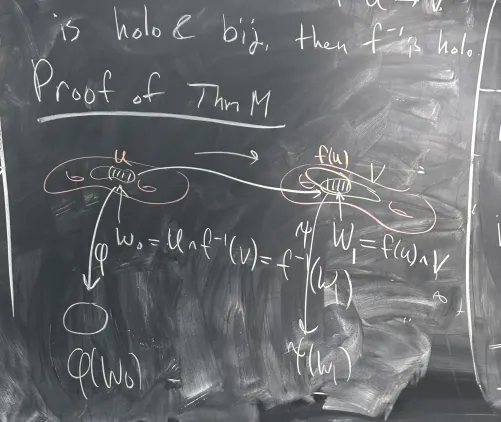
\includegraphics[width=0.5\textwidth]{Figures/cft-2.png},\]
    where the transition map from $\varphi(W_0)$ to $\psi(W_1)$ is bijective and holomorphic, so the inverse is holomorphic.
\end{proof}

\begin{example}[The Torus]
    Let $\Lambda = \Zbb + \Zbb \tau$ be a lattice in $\Cbb$, and let $X = \Cbb/\Lambda$ (in the sense that $\Lambda$ is a subgroup of $\Cbb$) and $\Lambda$ has a natural group action on $\Cbb$ by $(w, z) \in \Lambda \times \Cbb \to z + w$. We say that $z \sim z'$ if and only if there exists $w \in \Lambda$ such that $z' = z + w$.\\

    What are the charts of $X = \Cbb/\Lambda$? Suppose $U \subseteq \Cbb$ is open and $U \cap (U + w)$ is empty for all $w \in \Lambda$, then let $\Hat{U} = \{z + \Lambda\ |\ z \in U\} \subseteq X$. Then we can define $\varphi: \Hat{U} \to \Cbb$ defined by just $\varphi(z + \Lambda) = z$ for $z \in U$. The $\Hat{U}$ forms an open cover of the quotient space as we vary $U$ around satisfying the constraint.\\

    Finally, for any two charts $\varphi_0: \Hat{U_0} \to \Cbb$ and $\varphi_1: \Hat{U_1} \to \Cbb$, then $\varphi_1 \circ \varphi_0^{-1}$ is a translation map of the domain by an element of the lattice and is thus holomorphic.
\end{example}

\begin{example}[A Non-Hausdorff ``Riemann Surface"]
    Let $f(z) = z^2$ for $z \in A(r, 1)$ where $0 < r < 1$ and $A(r, 1)$ denotes the open annulus. Write $z_0 \sim z_1$ if there exists $k, \ell$ such that $f^k(z_0) = f^\ell(z_0)$ (the power here means composition). In other words, $f^k(z) = z^{2^k}$. Note that this is just the transitive closure of specifying $z \sim f(z) = z^2$.\\

    It turns out that $X = A(r, 1)/\sim$ satisfies all axioms of a Riemann Surface except being Hausdorff.
\end{example}

\newpage
\section{Lecture January 30th}

\textbf{Announcement:} Starting this Friday, you will be invited to submit 1 or 2 problems to the instructor from review, either from the notes or created by yourself! For making up questions yourself, the idea would be to answer questions that you have found over this course!!!! If it's from another source, you should absolutely cite it.

Recall from last time that - A Riemann surface $(X, \{\varphi_\alpha: U_\alpha \to \Cbb\})$ is a topological space $X$ with charts $\varphi_\alpha: U_\alpha \to \Cbb$ such that
\begin{itemize}
    \item $X$ is Hausdorff.
    \item The collection of $U_\alpha$ forms an open cover of $X$.
    \item For each $\alpha$, $\varphi_\alpha: U_\alpha \to \Cbb$ is a homeomorphic onto its image whose image is open in $\Cbb$.
    \item For all $\alpha$ and $\beta$, $\varphi_\beta \circ \varphi_\alpha^{-1}$ is holomorphic everywhere defined.
    \item $X$ is second countable (equivalently this follows from a deep theorem if $\{U_\alpha\}$ is countable).
    \item $X$ is connected. (otherwise $X$ is a complex $1$-manifold).
\end{itemize}

There are some slight \textbf{variations}:
\begin{itemize}
    \item If we let $\varphi_\beta \circ \varphi_{\alpha}^{-1}$ be smooth, then $X$ is a smooth surface.
    \item We can take $\varphi_\alpha: U_\alpha \to \Cbb^n$ and get a complex $n$-manifold (we do need to, however, define what a holomorphic map is between $\Cbb^n$).
    \item We can take $\varphi_\alpha: U_\alpha \to \Rbb^n$ with smooth overlaps to get a smooth $n$-manifold.
\end{itemize}

Note that Property 5 (2nd countable) is equivalent, on a manifold, to paracompact, which is equivalent to being metrizable. What's special about Riemann Surfaces are that Property $1, 2, 3, 4, 6$ actually implies Property $5$.

\subsection{Genus and Ends}

\begin{definition}
    An invertible linear map $T: \Rbb^n \to \Rbb^n$ is orientation-preserving if $\det(T) > 0$. It is orientation-reversing if $\det(T) < 0$.
\end{definition}

In particular, if $f: U \to \Cbb$ is holomorphic, then we can think of this a s a map $\hat{f}: U \subseteq \Rbb^2 \to \Rbb^2$. In this case, $D \hat{f}_z$ is orientation preserving because the derivative is of the form
\[\begin{pmatrix}
    u & v\\
    -v & u
\end{pmatrix},\]
by the Cauchy-Riemann equations, with determinant of the form $\det D\hat{f}_z = u^2 + v^2 > 0$ (as long as $f'(z) \neq 0$).\\

\begin{definition}
    A smooth $n$-manifold is \textbf{oriented} when given charts with $\det D_x(\varphi_\beta \circ \varphi_\alpha^{-1}) > 0$.
\end{definition}

In particular, this implies that
\begin{proposition}
    A Riemann Surface is always oriented.
\end{proposition}

First we restrict our attention to smooth surfaces. Let $X$ be a smooth orientable surface, then,

\begin{definition}
    The \textbf{genus} of $X$ is the maximal number of disjoint simple closed curves on $X$ that does not disconnect $X$ if removed. It is possible for a surface to have infinite genus. We should probably require the curves to be smooth, but the number turns out to be the same even if it's just continuous. A surface is said to be \textbf{planar} if it has genus $0$.
\end{definition}

Here we assume the following background results on smooth manifolds that are known already
\begin{theorem}
    Any compact surfaces have finite genus. Furthermore, any two connected compact (orientable) surfaces of genus $g$ are diffeomorphic.
\end{theorem}

Now we will also introduce the notion of \textbf{ends}. Let $X$ again be a smooth orientable surface.
\begin{definition}
If $K \subseteq L \subseteq X$, then we get an inclusion $X \setminus L \to X \setminus K$, and then this gives a well-defined map $i_{LK}: \operatorname{Comp}(X \setminus L) \to \operatorname{Comp}(X \setminus K)$ where $\operatorname{Comp}$ refers to connected components (thought of as discrete topological spaces).\\

Then we define $\mathcal{E}(X)$ (``space of ends of $X$") be the inverse limit
\[\varprojlim i_{KL}\]
indexed over all compact subsets $K \subseteq X$ in the following sense:
% https://q.uiver.app/#q=WzAsNCxbMSwxLCJcXG9wZXJhdG9ybmFtZXtDb21wfShYIFxcc2V0bWludXMgTCkiXSxbMSwyLCJcXG9wZXJhdG9ybmFtZXtDb21wfShYIFxcc2V0bWludXMgSykiXSxbMCwwLCJcXG1hdGhjYWx7RX0oWCkiXSxbMSwwLCIuLi4iXSxbMiwwXSxbMiwxXSxbMCwxXSxbMiwzXSxbMywwXV0=
\[\begin{tikzcd}
	{\mathcal{E}(X)} & {...} \\
	& {\operatorname{Comp}(X \setminus L)} \\
	& {\operatorname{Comp}(X \setminus K)}
	\arrow[from=1-1, to=2-2]
	\arrow[from=1-1, to=3-2]
	\arrow[from=2-2, to=3-2]
	\arrow[from=1-1, to=1-2]
	\arrow[from=1-2, to=2-2]
\end{tikzcd}\]
Here's an alternative more concrete characterization - for each $e \in \mathcal{E}(X)$ and compact $K \subseteq X$, we get $e_K \in \operatorname{Comp}(X \setminus K)$ (by the map given in universal property). Hence we can think of $e$ as a choice of component in $X \setminus K$. Furthermore, this satisfies
\[i_{LK}(e_L) = e_K.\]
So it's the set of choices of components that are consistent with respect to inclusion $X - L \to X - K$. The base for topology $B$ of $\mathcal{E}(X)$ in this case is
\[\Hat{U} = \{e \in \mathcal{E}(X)\ |\ e_K = U\},\]
where $U \in \operatorname{Comp}(X \setminus K)$.\\

$\mathcal{E}(X)$ is roughly ``ways you can go to $\infty$ in $X$". The concept works intelligently in locally compact spaces.
\end{definition}

\begin{example}
    Here are some example of ends,
    \begin{itemize}
        \item  Note that if $X$ is compact, then $\mathcal{E}(X)$ is empty.
        \item For an infinite cylinder $S^1 \times \Rbb$, there are two ends at infinity.
        \item This surface $X$ actually only has one end:
        \[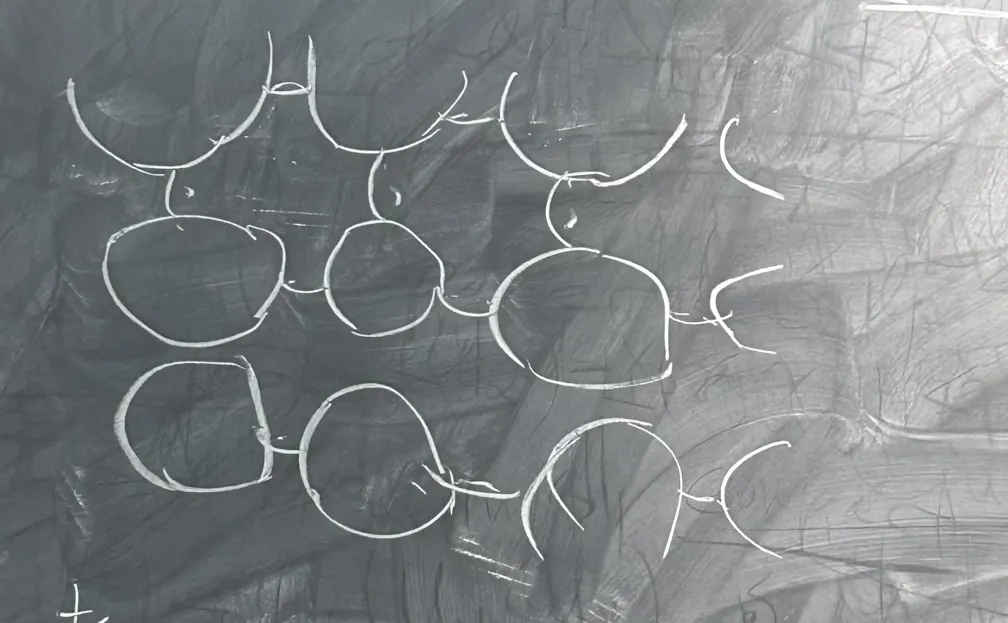
\includegraphics[width=0.6\textwidth]{Figures/lec2-1.png}\]
        This is because every way to go to infinity is equivalent to the complement of $X \cap \overline{B}_{R}(0)$ as $R$ gets larger.
        \item $\Cbb \setminus \{\text{n points}\}$ has $n+1$ ends. $\Cbb$ itself has $1$ end at infinity.
    \end{itemize}
\end{example}

\begin{exercise}
    If $X$ is a surface and $A \subseteq X$ is compact, $\mathcal{E}(X \setminus A) \equiv \mathcal{E}(X) \sqcup \operatorname{Comp}(A)$ (canonically homeomorphic).
\end{exercise}

\begin{exercise}
    If $X$ is a surface, then $X \sqcup \mathcal{E}(X)$ is compact, the topology here is $U = U_X \cup \{\Hat{U} \subseteq \mathcal{E}(X) \text{ union } U \subseteq X, \text{ for each } U \in \operatorname{Comp}(X \setminus K)\}$. Furthermore, $\mathcal{E}(X) \subseteq X \sqcup \mathcal{E}(X)$ is closed under the given topology (this sort of follows immediately because the definition requires any open subset of $X$ to be open in the disjoint union, including $X$ itself).
\end{exercise}

Note that $X_n \to e$ for sequence $X_n \in X$ and $e \in \mathcal{E}(X)$ if and only if for all compact $K \subseteq X$, $X_n \in e_K \in \operatorname{Comp}(X \setminus K)$ for all large $n$.

\begin{definition}
    An end is \textbf{planar} if has a \textbf{planar} (genus zero) neighborhood (take a compact set, see which component the end takes in the complement). Note that the set of planar ends $\mathcal{P}(X)$ are open.
\end{definition}

For example, this has two ends,
\[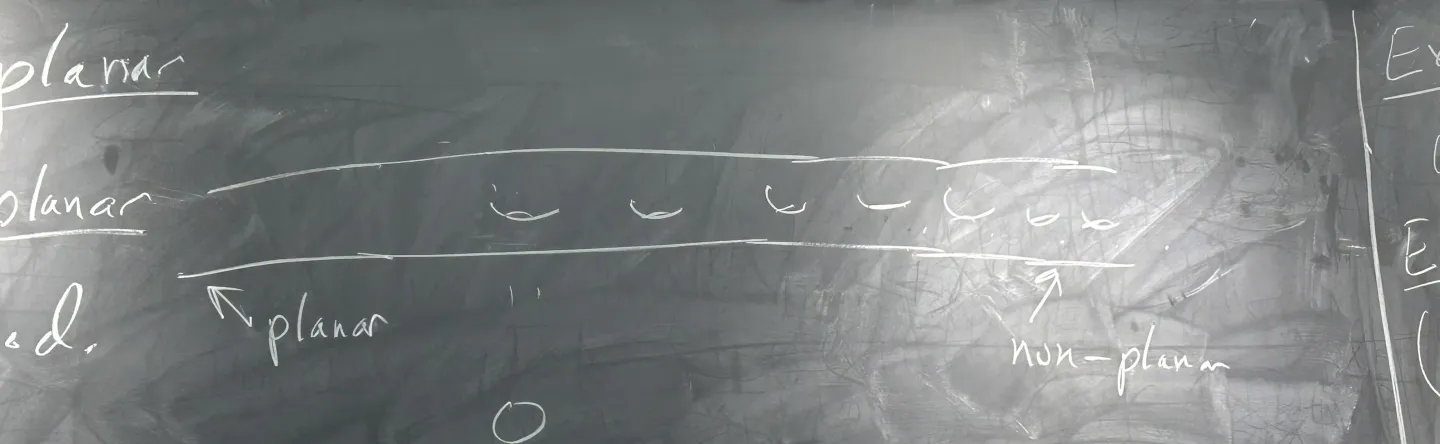
\includegraphics[width=0.6\textwidth]{Figures/lec2-2.png}\]
The left side is planar. The right side is not planar.\\

Given $X$, we get the genus $g(X) \subseteq \Nbb \cup \{\infty\}$, ends $\mathcal{E}(X)$, and $\mathcal{P}(X) \subseteq \mathcal{E}(X)$ open. The amazing theorem we get is that
\begin{theorem}
    For all triples $(g, \mathcal{E}, \mathcal{P})$ with $\mathcal{E}$ totally disconnected, metrizable, and compact, $\mathcal{P}(X) \subseteq \mathcal{E}(X)$ open with $P = \mathcal{E}$ if $g < \infty$. Then there exists a surface $X$ with these invariants unique up to diffeomorphism. 
\end{theorem}

\newpage
\section{Lecture February 1st}

\subsection{Pullback of Riemann Surface Structure}

Let $f: X \to Y$ be a continuous map, we say it's a local homeomorphism if for all $x \in X$, there exists $U \subseteq X$ containing $x$ and $V \subseteq Y$ (U, V open), such that $f$ is a homeomorphism of $U$ onto $V$.

\begin{theorem}
Suppose $Y$ is a Riemann Surface, and $X$ is connected and Hausdorff, and $f: X \to Y$ is a local homeomorphism, then there exists a unique Riemannian surface structures on $X$ such that $f: X \to Y$ is then holomorphic.\\

By the existence of Riemann surface structure, we mean a collection of charts $\varphi_\alpha: U_\alpha \to \Cbb$ on $X$.\\

By the uniqueness of Riemann surface structure, we mean that the overlap/transition function on the combination of all charts are still holomorphic (equivalently, they are contained in the same maximal atlas). More equivalently, let $\sigma$ and $\tau$ be two Riemannian surface structures on $X$, then the identity map
\[(X, \sigma) \to (X, \tau)\]
is a holomorphic map.
\end{theorem}

\begin{remark}
    In particular, any covering space $\rho: X \to Y$ will satisfy the description above, hence covering spaces of Riemann surfaces have unique Riemann surface structures.
\end{remark}

\begin{remark}
    Given $X$ and a Riemannian surface structure $\sigma$ with charts $\varphi_\alpha: U_\alpha \to \Cbb$. Let $\operatorname{conj}: \Cbb \to \Cbb$ be the complex conjugation map, then define charts $\psi_\alpha = \operatorname{conj} \circ \varphi_\alpha$, this gives a Riemannian surface structure $\tau$ on $X$. In this case, the identity map
    \[id: (X, \sigma) \to (X, \tau)\]
    is \textbf{anti-holomorphic}.
\end{remark}

\begin{proof}[Proof of the Theorem]
    Let $x \in X$, let $(U, V)$ be the pair of open sets in $X$ and $Y$ respectively under the local homeomorphism hypothesis. Without loss of generality (taking intersection with charts of $Y$), we can assume that there's a chart $\psi: V \to \Cbb$, then we define a map $\phi: U \to \Cbb$ such that
    \[\phi = \psi \circ f,\]
    then it's a routine exercise to verify that the charts on $X$ gives it a Riemannian surface structure (since $X$ is already connected and Hausdorff), and that $f$ is holomorphic.\\
    
    The only issue with this proof is that we DID NOT assume that $X$ is second countable. Now it is a very deep theorem (as we said before) that all the other conditions imply that $X$ is second countable, but that's a very big result.\\

    For uniqueness, use the fact that $f$ is a local homeomorphism to try to construct an identity map on $X$ that is holomorphic.
\end{proof}

\begin{exercise}[Student is encouraged to do this...]
    Prove $X$ has holomorphic overlaps and $f: X \to Y$ is holomorphic.
\end{exercise}

\begin{exercise}
    Assume that $X$ is 2nd countable, or does it follow?
\end{exercise}

\subsection{Local Branched Cover of Oriented Surfaces}

\textbf{Motivation:} Consider the map $z \mapsto z^n$ on the unit disk $\mathbb{D} \subseteq \Cbb$, then this gives an degree $n$ covering map $\mathbb{D} - \{0\} \to \mathbb{D} - \{0\}$.

\begin{definition}
    Between oriented surfaces, $f: X \to Y$ (continuous map) is a branched cover if for all $x$, there exists open $U \subseteq X$ containing $x$, $V \subseteq Y$ containing $f(x)$ (both $U$ and $V$ are topological disks) such that
    \begin{itemize}
        \item $f: U \setminus \{x\} \to Y \setminus \{f(x)\}$  is a proper local homeomorphism. (note that if the degree is $n < \infty$, then it is actually topologically equivalent to what we said in the Motivation).
    \end{itemize}
\end{definition}

There's a brief lemma we glossed over in the definition above we need to justify:
\begin{lemma}[Lemma B]
    Let $U$ and $V$ be topological disks and $f: U \to V$ is continuous. Suppose f restricted to $U \setminus \{x\} \to V \setminus \{f(x)\}$ is a proper local homeomorphism (which is a finite sheeted covering map, with degree say $n$), then there exists $h_U, h_V$ homeomorphisms to the disk such that the diagram commutes:
    % https://q.uiver.app/#q=WzAsNCxbMCwwLCJVIl0sWzIsMCwiViJdLFswLDIsIlxcbWF0aGJie0R9Il0sWzIsMiwiXFxtYXRoYmJ7RH0iXSxbMCwyLCJoX1UiXSxbMCwxLCJmIl0sWzEsMywiaF9WIiwyXSxbMiwzLCJ6IFxcbWFwc3RvIHpebiJdXQ==
\[\begin{tikzcd}
	U && V \\
	\\
	{\mathbb{D}} && {\mathbb{D}}
	\arrow["{h_U}", from=1-1, to=3-1]
	\arrow["f", from=1-1, to=1-3]
	\arrow["{h_V}"', from=1-3, to=3-3]
	\arrow["{z \mapsto z^n}", from=3-1, to=3-3]
\end{tikzcd}\]
\end{lemma}

Here's another topological fact
\begin{exercise}
    Let $g: X \to Y$ be a proper local homeomorphism between surfaces, then $g$ is a finite-sheeted cover.
\end{exercise}

\begin{proof}[Proof of Lemma B]
    Take $h_V$ with $h_V(f(x)) = 0$ (by a Mobius transformation), then we lift $h_V \circ f$ by $z \mapsto z^n$ where $n = \operatorname{deg}(f)$ on $U - \{x\}$. So $h_V \circ f$ and $(z \mapsto z^n)$ are both covering maps that have the same image (in terms of fundamental groups), so from covering space theory we can lift $h_V \circ f$ to give a covering map $h_U: U \to \mathbb{D}$ that makes the diagram commute:
    \[\begin{tikzcd}
	U && V \\
	\\
	{\mathbb{D}} && {\mathbb{D}}
	\arrow["{h_U}", from=1-1, to=3-1]
	\arrow["f", from=1-1, to=1-3]
	\arrow["{h_V}"', from=1-3, to=3-3]
	\arrow["{z \mapsto z^n}", from=3-1, to=3-3]
\end{tikzcd},\]
then one can check that $h_U$ is a homeomorphism.\\

\textbf{Exercise:} Fill in the details of this proof.
\end{proof}

Now we have reached a new theorem:
\begin{theorem}
    If $Y$ is a Riemann surface and $f: X \to Y$ is a local branched cover, and $X$ is connected and Hausdorff (and second countable), then there exists an unique Riemann surface structure on $X$ such that $f: X \to Y$ is holomorphic.
\end{theorem}

\begin{proof}
    First observe that the set $B \subseteq X$ of \textbf{branched points} (the points where $f$ is not a local homeomorphism) is discrete, then $f: X \setminus B \to Y$ is a local homeomorphism. Since $B$ is discrete, $X \setminus B$ is still RS, and the previous theorem tells us that there exists an unique Riemann surface structure on $X \setminus B$.\\

    For each $x \in B$, we can use $h_{U}: \hat{U} \to \mathbb{D}$ where given by Lemma B, where $h_V: \hat{V} \to \mathbb{D}$ is a holomorphic homeomorphism (after possible intersection with the charts already given and taking pre-images - essentially we are shrinking $U, V$ until we get into holomorphic charts).\\

    Here's an illustrative diagram indicating roughly what's happening in the discussion above:
\[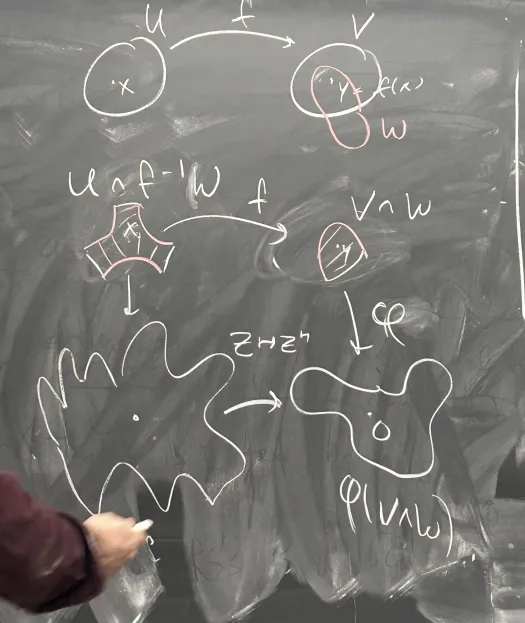
\includegraphics[width=0.4\textwidth]{Figures/lec3-1.png}\]

    The branched points are discrete because each point is isolated because $f$ is supposed to be a local homeomorphism on $N - \{p\}$ in a neighborhood $N$ containing the branch point $p$.\\

    \textbf{Exercise: } Verify holomorphic and explain $\hat{U}$.\\

    For uniqueness of the Riemannian Surface structure, given two structures near $X$, \underline{lift} $f$ near $X$ \underline{by} $f$ to get that the identity map of $U \setminus \{x\}$ is holomorphic, and by the Riemann removable singularity theorem, it is holomorphic on $U$.
\end{proof}

In fact, there's another theorem:
\begin{theorem}
    Every non-constant holomorphic map of Riemann surfaces is a local branched cover.
\end{theorem}

\subsection{Building Riemann Surfaces}
So far, we haven't built that much Riemann Surfaces yet, but we can now try to build some with the theorems given.\\

Suppose $E \subseteq Y$ is a discrete subset of a Riemann Surface (sometimes called the branched values), then take $H$ a subgroup of $\pi_1(Y \setminus E)$ of finite index $n$. Galois correspondence tells us that there exists a degree $n$ covering map from $g: X' \to Y \setminus E$. Near each $y \in E$, we get this finite covering map $g: U' \to V - \{y\}$, where $U', V$ are appropriately small disks.\\

\textbf{Claim: } We can fill in each $U'$ to make $U$ such that $g: U \to V$ is a local branched cover (and we also complete $X'$ to $X$), and then $g: X \to Y$ is a (global) branched cover.\\

\textbf{Note: } A global branched cover have several definitions that agree on a finite sheeted cover, but we will settle to one of them in the case of finite sheeted cover:
\begin{itemize}
    \item For all $y \in Y$, there exists $V \equiv V_y \subseteq Y$ containing $y$ such that $g$ on each component $U_i$ of $g^{-1}(V)$ gives:
    \item There exists $x_i \in U_i$ with $g^{-1}(y) \cap \{U_i\} = \{x_i\}$, and $g: U_i - \{x_i\} \to V - \{y\}$ is a proper local homeomorphism.
    \item See the following illustrate picture
\[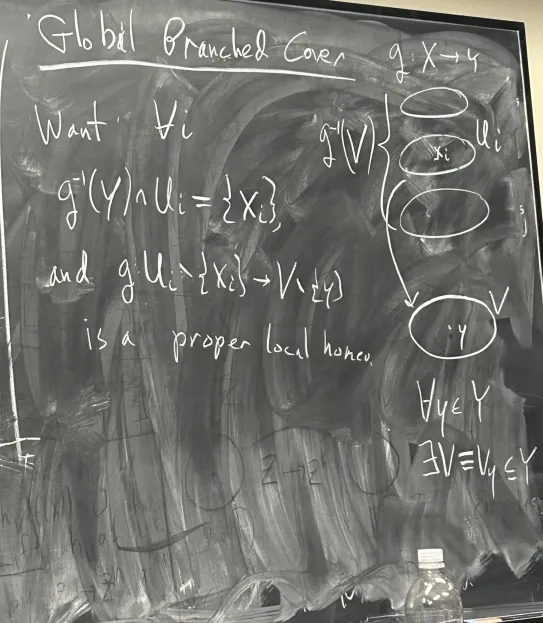
\includegraphics[width=0.4\textwidth]{Figures/lec3-2.png}\]
\end{itemize}

\begin{question}
    How can we fill $U'$ to $U$?
\end{question}

Well, locally we have that $U, V$ is homeomorphic to $\mathbb{D} \setminus \{0\}$ and the map behaves like $z \mapsto z^n$, we want to then continuously extend the homeomorphism to the origin and then lift that to $\mathcal{E}(U')$ to be added to $U'$. Even without considering ends, we could do something like
\[X' \sqcup \mathbb{D} / h_{U'}\]
via an appropriate quotient map. Please see the following illustrative picture:
\[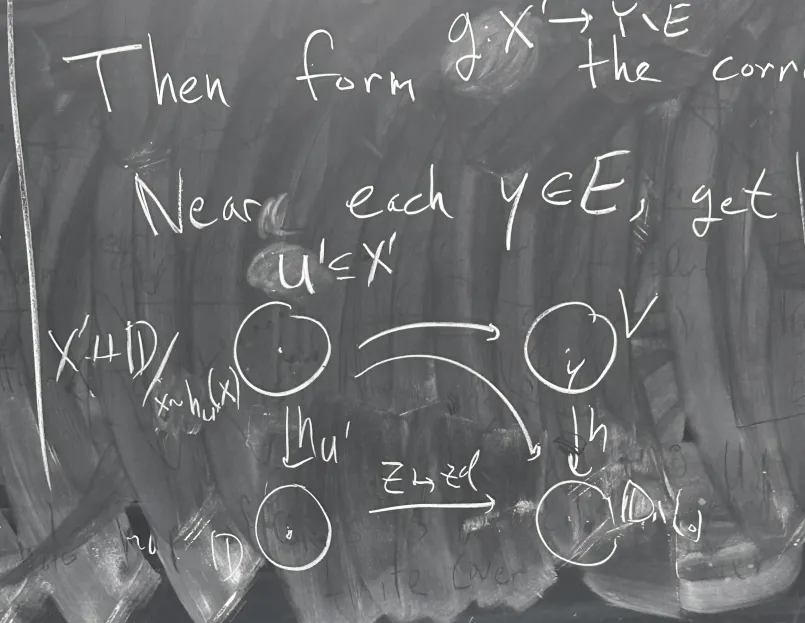
\includegraphics[width=0.5\textwidth]{Figures/lec3-3.png}\]

\newpage
\section{Lecture February 6th}

\subsection{Possibly Large Riemann Surfaces}

\begin{definition}
    A \textbf{possibly large} Riemann Surface $X$ is one where $X$ satisfies all axioms except (possibly) 2nd countable. Of course, by Rado's Theorem, we will see later that all possibly large Riemann surfaces are second countable, but we would like to work without this assumption yet.
\end{definition}

This definition is motivated because we actually figured out the questions bugging us last time:
\begin{theorem}[Poincare-Volterra Theorem]
    Suppose $f: X \to Y$ is a local homeomorphism (or local branched cover) of possibly large surfaces, and $Y$ is second countable, then $X$ is second countable.
\end{theorem}

\begin{remark}
    The theorem above is not Poincare-Volterra Theorem in its full generality but rather only a special case.
\end{remark}

\begin{proof}
The proof is divided into the following steps:
\begin{enumerate}
    \item As an exercise, we note that a Riemann surface is second countable if and only if it admits a countable cover by charts (that in fact forms a basis).
    \item Since $Y$ is second countable, let $W = \{W_i\}$ be a countable cover of $Y$ of connected charts.
    \item Let $\mathcal{V} = \{V \subseteq X\ |\ f(V) \in W \text{ and } f: V \to f(V) \text{ is a homeomorphism}\}$. We see that $\mathcal{V}$ is actually a base for topology on $X$, the idea is that - given any $x \in X$, we can find a neighborhood of $x$ that's mapped homeomorphically into $Y$, we then find a neighborhood around the image given by $W_i$ that pullback to a base for topology.
    \item \textbf{Claim: } $\mathcal{V}$ is a countable set. B.  For all $V \in \mathcal{V}$, the set $\{V' \in \mathcal{V}\ |\ V \cap V' \neq \emptyset\}$ (where $V$ is fixed) is countable. Indeed, consider the function $f$ restricted to each neighborhoods in the set $\{V' \in \mathcal{V}\ |\ V \cap V' \neq \emptyset\}$ is countable-to-1. \mattie{what}
    \item C. Choose $V_0 \in \mathcal{V}$, let $\mathcal{V}_0 = \{V_0\}$, and generally we construct
    \[\mathcal{V}_{k+1} = \{V \in \mathcal{V}\ |\ \exists V' \in \mathcal{V}_k \text{ such that } V \cap V' \neq \emptyset\}.\]
    The picture to have in mind is everything you can reach in $k+1$ steps:
    \[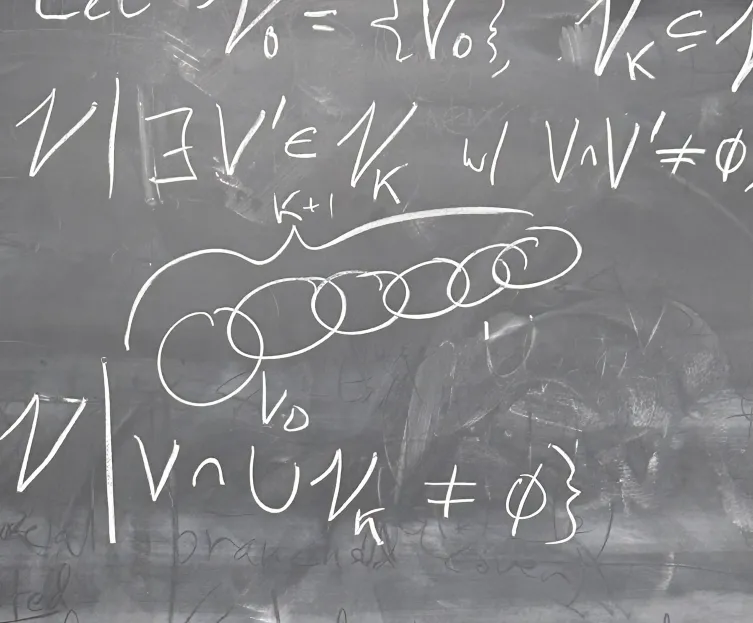
\includegraphics[width=0.5\textwidth]{Figures/lec4-1.png}\]
    Equivalently $V_{k+1}$ is the set
    \[\mathcal{V}_{k+1} = \{V \in \mathcal{V}\ |\ V \cap \bigcup_{i = 1}^k \mathcal{V}_k \neq \emptyset\}\]
    \item Then $\mathcal{V}_k$ is countable by B and induction. Hence we have that
    \[\mathcal{V}_\infty = \bigcup_{k = 0}^\infty \mathcal{V}_k\]
    is countable. Note that we haven't used connectedness yet.
    \item D. We claim that the union $\bigcup_{V \in \mathcal{V}_\infty} V = X$ (\textbf{Notaton:} We use $\bigcup \mathcal{V}_\infty$ to denote the union $\bigcup_{V \in \mathcal{V}_\infty} V$, this is a notation from set theory that is adopted here.) 
    \begin{proof}[Proof of D]
        If this is not the case, then $\mathcal{V}_\infty \subsetneq \mathcal{V}$ and $X \setminus \bigcup \mathcal{V}_\infty = \bigcup (\mathcal{V} - \mathcal{V}_\infty)$. Then $\bigcup \mathcal{V}_\infty$ and $X \setminus \bigcup \mathcal{V}_\infty$ are both open disjoint non-empty sets, so $X$ would be disconnected!
    \end{proof}
    \item Thus $\bigcup_{V \in \mathcal{V}_\infty} V = X$ so $X$ can be covered by countable neighborhoods.
\end{enumerate}
\end{proof}

Last time, we were also constructing examples of Riemann surfaces.
\begin{example}
    Let $E \subseteq \hat{\Cbb}$ be finite, let $H \setminus \pi_1(\hat{\Cbb} \setminus E)$ be a subgroup of finite index. Then we get a finite-sheeted cover $\hat{X}$ of $\hat{\Cbb} \setminus E$ that can be filled into a covering map $\pi: X \to \hat{\Cbb}$ with $\pi: X \to \hat{\Cbb}$ with $\pi$ as a branched cover and $X$ is compact.\\

    To make this notion rigorous, we should develop some more discussion about ends. Indeed, for a general surface $X$, for all $e \in \mathcal{E}(X)$, there exists $\alpha: [0, 1) \to X$ with $\lim_{t \to 1} \alpha(t) = e$, with the properties:
    \begin{itemize}
        \item Every proper path in $X$ limits to a unique end (proper here means $\alpha^{-1}(K)$ is compact for all compact $K \in X$). 
        \item Properly paths are properly homotopic implies they limit to the same end. By \textbf{properly homotopic}, we mean that for $\alpha_0, \alpha_1: [0, 1) \to X$, then a proper homotopy is - $\alpha: [0, 1] \times [0, 1)$ where we write $\alpha(s, t) = \alpha_s(t)$ where $\alpha$ is proper. (NOTE THAT WE DO NOT REQUIRE $\alpha$ to fix end points). 
        \item If the ends are isolated, the converse is also true (probably, the instructor's a bit unsure).
    \end{itemize}
    We could use these discussion of proper paths to do the extension mentioned in the example.
\end{example}

\begin{remark}
    There is a discussion of everything talked about here for review in the first 5 sections of Forster.
\end{remark}

\subsection{Hyperelliptic Covers}

\begin{proposition}
Now suppose that $F \subseteq \widehat{\Cbb}$ has even cardinality, then there exists a unique ($X$, $g: X \to \widehat{\Cbb}$) such that $g$ is a \textbf{holomorphic degree $2$ branched cover}, branched exactly over the points of $F$.    
\end{proposition}

This is what's called a \textbf{hyperelliptic cover}. This theorem essentially classifies all degree $2$ cover over $\widehat{\Cbb)$ based on its branch values.

\begin{proof}
\begin{enumerate}
    \item What is $\pi_1(\widehat{\Cbb} \setminus F)$? It is the free group of rank $2k - 1$. More geometrically it is also the group
    \[\langle g_1, ..., g_{2k}\ |\ g_1 ... g_{2k} = 1\rangle\]
    \item What are the subgroup $H$ of $\pi_1(\widehat{\Cbb} \setminus F)$ with index $2$? We first note all index $2$ subgroups are normal, the only order $2$ group is $\Zbb/2\Zbb$. In other words, all index $2$ normal subgroups are kernels of the homomorphism
    \[h: F_{2k - 1} \to \Zbb/(2\Zbb)\]
    How many such homomorphisms are there? Well, there are exactly $2^{2k-1}$ of them, based on what they send the generators to.
    \item Given some $h: F_{2k-1} \to \Zbb/2\Zbb$, what are the points that $h$ is branched over? Indeed, it's exactly the $z_i = h(g_i) = 1 \in \Zbb/2\Zbb$.
    \item What about the point at infinity? Topologically this happens, when we have a curve over the point at infinity. This happens when $h(g_i) = 1$ for all $i$.
    \item This is because $h(g_{2k}) = \sum_{i = 1}^{2k-1} h(g_i)$
    \item Therefore, there's only one unique branched cover with the constraint
    \[h(g_1) = ... = h(g_{2k-1}) = 1\]
\end{enumerate}
Note: To be branched over a point means - if you start with a point - it means one of these $n_i$ has to be greater than $1$
\end{proof}

\subsection{Geometric Realization of the Hyperelliptic Cover}
Here's also a more geometric perspective on what is happening:\\

Specifically, suppose that $E \subseteq \widehat{\Cbb}$ has even cardinality, and let ($X$, $g: X \to \widehat{\Cbb}$) be the branched double cover over $\widehat{\Cbb}$ branched at $E$. Note that we never explicitly spelled out what the hyper-elliptic cover $X$ is look.

Here we give an explicit construction of what $X$ is. Indeed, $X$ maybe constructed explicitly as follows.\\

Let $|E| = 2n$ for $n \geq 1$, and let $Y$ be the genus $n-1$ surface as follows:
\[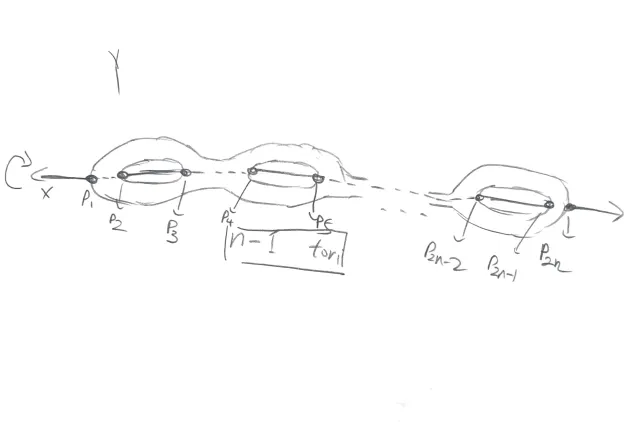
\includegraphics[width=0.6\textwidth]{Figures/hyper.png}\]
Although the diagram is not perfect, you should think of the $x$-axis as straight and $Y$ as being symmetric with respect to the $x$-axis.\\

Now consider the group action $\Zbb/2\Zbb$ on $Y$ given by rotating along the $x$-axis by $180$ degrees. Then this action will have orbit of size $2$ for every point on $Y$ except for $p_1, ...., p_{2n}$ labeled. The set $\{p_1, ..., p_{2n}\}$ are the fixed point of this group action (ie. they have orbit one).\\

Hence, we obtain a degree $2$ branched cover $p: Y \to Y/G$ branched at exactly $\{p_1, ..., p_{2n}\}$. Furthermore, if you examine what $Y/G$ is, it would be $\hat{\Cbb}$. One could deduce this from more rigorous arguments but just investigate what points gets glued to which, the resulting surface in the quotient will have genus $0$.\\

Thus, we have that the hyperelliptic double covers discussed in classes are homeomorphic to a genus $n-1$ surface. This also shows that we can give a Riemann surface structure of any closed surface of genus $g$ by considering this branched cover.



\newpage
\section{Lecture February 8th}

\textbf{Office Hour: } Thursday 4 - 5 pm (or by appointment).\\

From last time, for the hyperelliptic cover. Consider $E \subseteq \hat{\Cbb}$ be a finite set of even points and $\infty \in E$. Write $\hat{E} = E - \infty$, then consider the map
\[q: \pi_1(\Cbb \setminus E') \to \Zbb/2\Zbb\]
by sending $\alpha_i \to 1$ where each $\alpha_i$ is a generator of $\pi_1(\Cbb \setminus E') \cong F^{2k-1}$ (free group on odd many generators).\\

 This gives an index $2$ subgroup $H = \ker(q)$ in $\pi_1(\Cbb \setminus E)$. If any of the $\alpha_i$ has $h(\alpha_i) = 0$, then it means that when we loop around the puncture given by $\alpha_i$, we are not switching branches, so the covering space is not branched over $\alpha_i$. Since $|E'|$ is odd, then the sum of all $q(\alpha_i)$ is $1$ modulo $2$ (which guarantees that it's branched over infinity - this is because a loop around infinity is freely homotopic to a loop going around all the points $\alpha_i$'s, and we ignore minus signs because it is mod $2$).

 \subsection{Riemann Surfaces and Analytic Continuations}

 \begin{definition}
     If $f_0: U_0 \to \Cbb$ and $f_1: U_1 \to \Cbb$ are holomorphic ($U_0, U_1$ are open), and $z \in U_0 \cap U_1$, then we say that $[f_0, z] = [f_1, z]$ (the \textbf{germ} of $f_0$ at $z$ if equal to the \textbf{germ} of $f_1$ at $z$) if there exists open $V \subseteq U_0 \cap U_1$ containing $z$ such that
     \[f_0|_V = f_1|_V.\]
     Note that by the identity theorem, this is equivalent to $f_0 = f_1$ on the component $W$ of $U_0 \cap U_1$ containing $z$.\\
     
     For $f: U \to \Cbb$ be holomorphic, we let $[f, U] = \{[f, z]\ |\ z \in U\}$ up to the equivalence class with the identification given above.\\

     From here we define $\mathcal{G}(\Cbb, \Cbb)$ (or more generally $\mathcal{G}(X, \Cbb)$ or $\mathcal{G}(X, Y)$ for Riemann surfaces) as
     \[\mathcal{G}(X, Y) = \{[f, x]\ |\ x \in U, f: U \subseteq X \to Y \text{ is holomorphic}\}.\]
     In this case $\{[f, U]\}$ is a base for the topology of $\mathcal{G}(X, Y)$.
 \end{definition}

In the last semester, we proved the following theorem
 \begin{theorem}[Fall 2023, Theorem 1]
     The space $\mathcal{G} \coloneqq \mathcal{G}(X, \Cbb)$ is Hausdorff. Furthermore, every component $Q$ of $\mathcal{G}$ has canonical local homeomorphism (projection by $[f, z] \to z$) $\pi: Q \to X$. (In fact, the projection $\pi: \mathcal{G} \to X$ is a local homeomorphism)\\
     
     Furthermore, our result from last week shows that each $Q$ has an unique Riemann surface structure as $\pi$ is a local homeomorphism making $\pi$ holomorphic. The very obvious Riemann surface structure is that $[f, U] \mapsto U$.
 \end{theorem}

 \begin{remark}
     $\mathcal{G}$ itself is not second countable.
 \end{remark}

We also had a second theorem.
\begin{theorem}[Fall 2023, Theorem 2, Monodromy Theorem]
    We are working in $\mathcal{G} = \mathcal{G}(X, \Cbb)$. If $\gamma_0, \gamma_1: I = [0, b] \to X$ (where $X$ is a Riemann Surface) are homotopic rel end points by a homotopy $\gamma_t: I \to X$ such that each $\gamma_t$ has a lift to $\mathcal{G}$ starting at $z_0$ ($\gamma_t(0) = z_0$ for all $t$).\\

    Then $\gamma_t(b)$ is constant independent of $t$. \mattie{explain wording}
\end{theorem}

\begin{question}
    When can we analytically continue along $\gamma$?
\end{question}

\begin{example}
    Suppose $f: \Cbb \to \Cbb$ is holomorphic, and $g: U \to \Cbb$ is a branch of $f^{-1}$ near $z_0 \in U$ (which just means that $g$ is holomorphic and $f \circ g = id$ on $U$). For instance, when $f(z) = e^z$, we could take $g(w) = \operatorname{Log} w$ to be on $\Cbb \setminus (-\infty, 0)$ where we take $-\pi < \operatorname{Im}(g(w)) < +\pi$.

    \begin{question}
        Take $\gamma: [0, b] \to \Cbb$ with $\gamma(0) = z_0$, when we can we analytically continue $g$ along $\gamma$?
    \end{question}

    In the special case with $f(z) = e^z$ as before. Let's pick $z_0 = 1$, so $g(z_0) = 0$. If the path we take crosses $(-\infty, 0)$, we would want to path to go out of $[-\pi, \pi]$.
    \[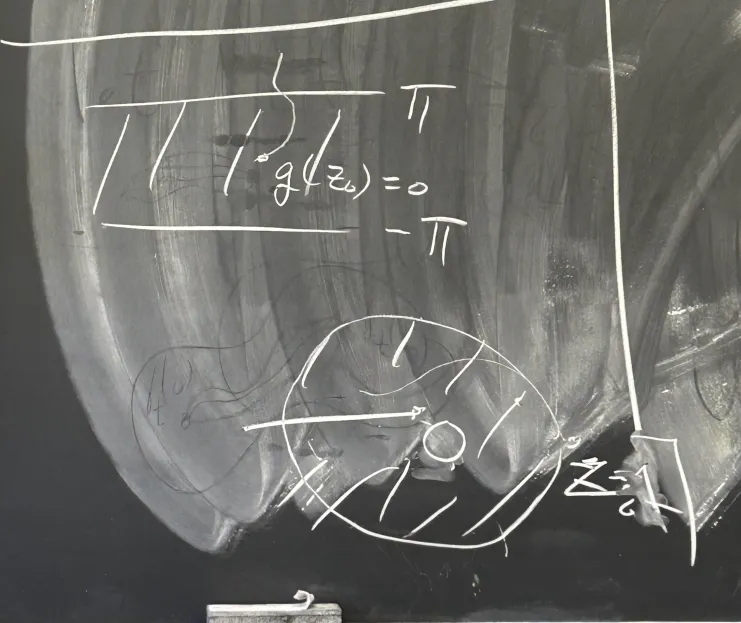
\includegraphics[width=0.5\textwidth]{Figures/lec5-1.png}\]
    More formally, $z \mapsto e^z: \Cbb \to \Cbb^*$ is a covering map, so we know that topologically we could always lift a path.
\end{example}

\begin{question}
    Another example is to consider $\sin: \Cbb \to \Cbb$, when can we analytically continue branch of $\sin^{-1}$?
\end{question}

Here's the general theory that may be able to help.
\begin{theorem}
    Suppose $f: U \subseteq \Cbb \to \Cbb$ is holomorphic and $\gamma: [0, b] \to \Cbb$. We can analytically continue along $\gamma$ starting from $g$ a branch of $f^{-1}$ near $\gamma(0) \in f(U)$ unless:
    \begin{itemize}
        \item There exist $0 \leq c \leq b$ such that $[0, c)$ is maximal interval for analytic continuation.
        \item And either (1) $g(\gamma(t)) \to $ critical point of $f$ or (2) $g(\gamma(t)) \to \infty$ in $U$ as $t \to c$ (we don't mean literal infinity, but to an end of $U$).
    \end{itemize}
\end{theorem}

Here's an example of how $(1)$ could occur:
\begin{example}
    Take $f(z) = z^2$ and it's ambiguous where lift the path past $\gamma(c) = 0$,
    \[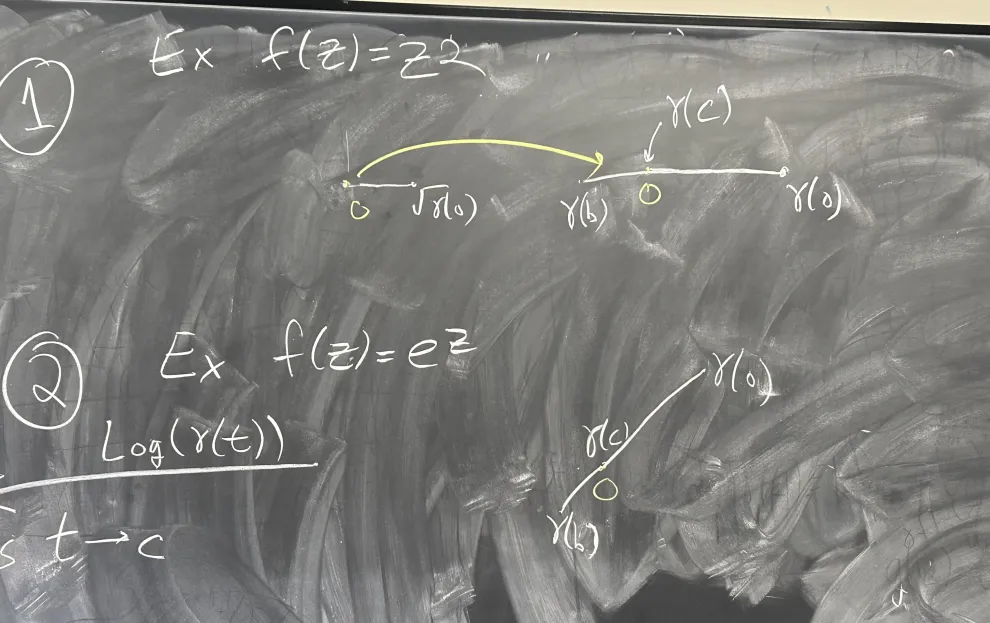
\includegraphics[width=0.5\textwidth]{Figures/lec5-2.png}\]
    This is because you are hitting a point where you don't really have a local inverse.
\end{example}

Here's an example of how $(2)$ could occur:
\begin{example}
    Take $f(z) = e^z$, then it's still ambiguous what happens at $\gamma(c) = 0$ (see the previous picture for a figure of this as well), because $\operatorname{Log}(\gamma(t))$ blows up at $t = c$. The caveat however is that $e^z$ will never hit $0$ for any value $z \in \Cbb$, so maybe this example is not that good, but it is going to infinity in the sense that it's going to an end.\\

    For clarity, let's consider the following example instead:
    \[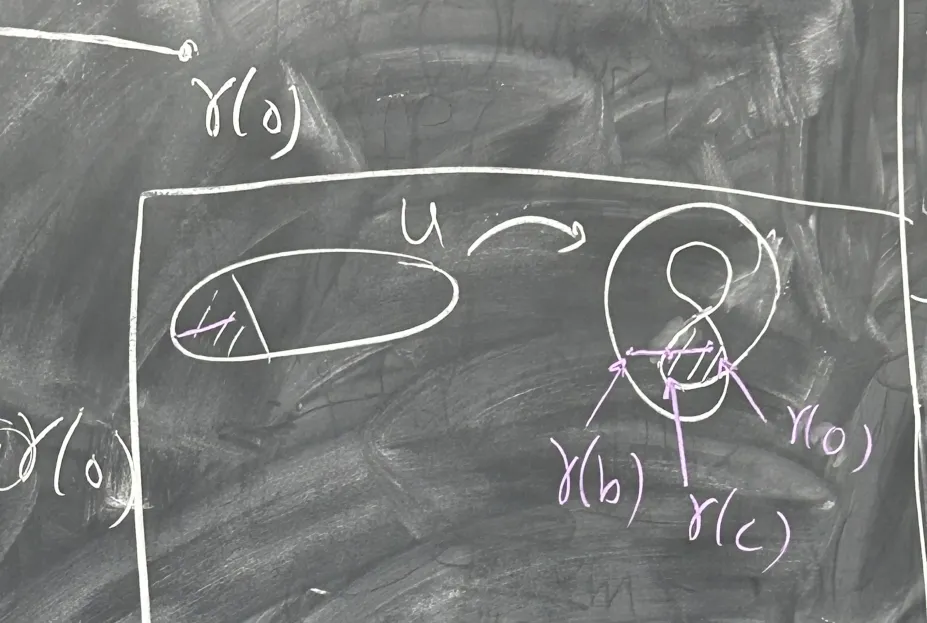
\includegraphics[width=0.5\textwidth]{Figures/lec5-3.png}\]
    where the path is also leaving $U$.
\end{example}

\begin{question}
    But what if we analytically continue $f$ itself outside of $U$? So, we really want to think of $U$ as an independent Riemann surface instead or assume it's the maximal analytic domain of $f$.
\end{question}

\textbf{NOTATION CHANGE:} Let's just assume $U = X$ is a Riemann surface instead.\\

\begin{definition}
    $\gamma(c)$ in Condition (1) is called a branch value or critical value. $\gamma(c)$ in Condition 2 is called an ``asymptotic value".
\end{definition}

\newpage
\section{Lecture Ferbuary 15th}

Recall from last lecture, we defined that
\begin{definition}
    Suppose $f: X \to Y$ is holomorphic, then $q \in Y$ is an \textbf{asymptotic value} of $f$ if there exists $\alpha: [0, \infty)$ continuous and proper, such that
    \[\lim_{t \to \infty} f(\alpha(t)) = q.\]
\end{definition}

\begin{example}
    Consider the function $f: \Cbb \to \Cbb$ given by $f(x) = e^{x}$, then we observe that $\lim_{t \to \infty} f(-t) = 0$. Note that $f$ has no continuous extension to $\hat{\Cbb}$, indeed if there is, then the extension $\hat{f}: \Cbb \cup \{\infty\} \to \Cbb \cup \{\infty\}$ would be a rational function. However, the function would have an essential singularity at $\infty$, which is a contradiction.
\end{example}

\begin{remark}
    As shown in the previous example, asymptotic values of $f$ doesn't match ends on $X$ to ends on $Y$.
\end{remark}

\begin{example}
    Consider the example $g(z) = \cos (z)$. We seek to find its crticial points, crtiical values, and asymptotic values.
    \begin{enumerate}
        \item \textbf{Critical Points:} $\{n \pi \ |\ n \in \Zbb\}$.
        \item \textbf{Critical Values:} $\{1, -1\}$.
        \item \textbf{Asymptotic Values:} We can write
        \[\cos(z) = \frac{e^{iz} + e^{-iz}}{2} = \cosh(iz), \text{ where } \cosh(z) = \frac{e^z + e^{-z}}{2}.\]
        Now we observe that
        \[\lim_{y \to \infty} \cos(iy) = \lim_{y \to \infty} \frac{e^{-y} + e^y}{2} = \infty,\]
        and hence that $|\cos(z)| \to \infty$ whenever $|\operatorname{Im} z| \to \infty$. Finally, for any $z = x + iy$,
        \begin{align*}
            \cos(x + yi) &= \cos(x) \cos(iy) - \sin(x) \sin(iy)\\
            &= \cos(x) \cosh(y) - i \sin(x) \sinh(y).
        \end{align*}
        Hence, $\cos(z)$ has no asymptotic values \mattie{what?}
    \end{enumerate}
\end{example}

The example above combined with the theorem we mentioned last lecture shows that
\begin{theorem}
    If $\alpha: [0, b] \to \Cbb \setminus \{1, -1\}$, then we can analytically continue any branch of $\cos^{-1}$ along $\alpha$ (or equivalently, this means that we can ``lift $\alpha$ by $\cos$").
\end{theorem}

\begin{exercise}
    Find a holomorphic function $f: \Cbb \to \Cbb$, such that $f$ is surjective and $0$ is an asymptotic value.
\end{exercise}

More generally, suppose $F: U \subseteq \Cbb^2 \to \Cbb$ is a holomorphic function (for example $F$ could be a complex polynomial in two variables), then we look at the connected components of 
\[V(F) \coloneqq \{(z, w) \ |\ F(z, w) = 0\}.\]
If $F$ is non-constant, then then by the identity theorem, its zero locus should have codimension $1$ in $\Cbb^2$ and we can think of it as a ``complex curve" with singular and smooth points:
\[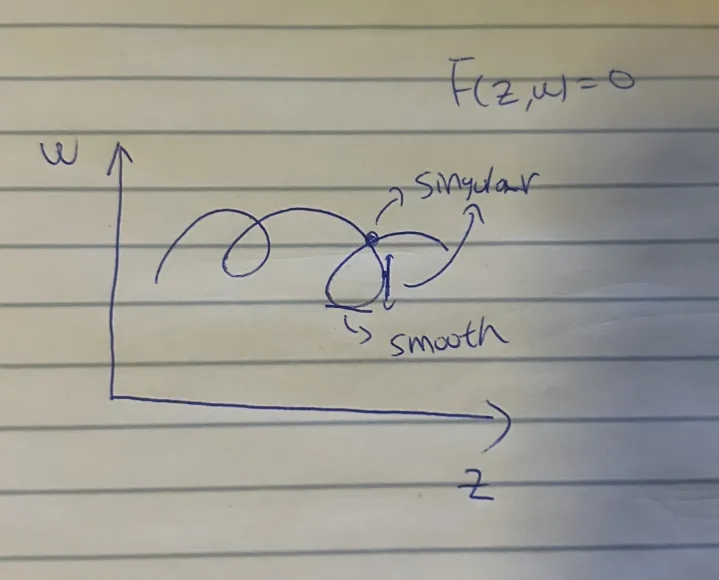
\includegraphics[width=0.5\textwidth]{Figures/lec6-1.png}.\]

Locally on $F(z, w) = 0$, we can parameterize $w = g(z)$ and consider $F(z, g(z)) = 0$. Then we hae that
\[0 = \frac{d}{dz} F(z, g(z)) = D_1 F + (D_2 F) g'(z).\]
Hence we can write
\[g'(z) = -\frac{D_1 F}{D_2 F}(z, g(z)).\]

\begin{question}
    Let $\alpha: [0, b] \to \Cbb$ be a branch of $g$ near $\alpha(0)$, when can we analytically continue along $\alpha$?
\end{question}

Note that if $D_2 F \neq 0$, we can apply the Inverse/Implicit Function Theorem for holomorphic functions to define $g(z)$ locally. If $D_2 F = 0$, then we can write $z = (w - w_0)^{n+1} + z_0$ for $F(z, w) = 0$ near $(z_0, w_0)$ for some power of $n$. \mattie{why talk about this?}\\

Hence, we can always analytically continue along $\alpha$ except when $D_2 F(z, g(z)) \to 0$ (ie. hitting a critical value) or $g(z) \to \infty$ for $z = \alpha(t)$ as $t \to t_0 \in [0, b)$ (ie. hitting an asymptotic value).

\begin{exercise}
    For a fixed $P(x, y) \in \Cbb[x, y]$, when can there be $\alpha: [0, 1] \to \Cbb^2$ such that
    \[P(\alpha(t)) \equiv 0, \]
    and $a^1(t) \to z_0 \in \Cbb$ and $a^2(t) \to \infty$ as $t \to 1$ ($a^1, a^2$ denotes the first and second coordinate of $\alpha$).
\end{exercise}

\begin{example}
    When $P(z, w) = zw - 1$, we could take $\alpha(t) = (1-t, \frac{1}{1-t})$.
\end{example}



\newpage
\section{Lecture Februrary 22nd}

\subsection{Meromorphic Functions}

Recall that for $U$ a domain in $\Cbb$, we say that $f$ on $U$ is a \textbf{meromorphic function} on $U$ if there exists $E \subseteq U$ that is discrete, such that $f: U \setminus \{E\} \to \Cbb$ is holomorphic, and $f$ has a pole at each point $e \in E$ (ie. the singularity should not be essential).\\

We can also think of $f$ as a holomorphic function $f: U \to \hat{\Cbb} = \Cbb \cup \{\infty\}$, and we take $E = f^{-1}(\{\infty\})$ to be discrete. 

\begin{definition}
    Let $X$ be a Riemann surface, we say a function $f$ on $X$ has \textbf{pole} (or removable singularity) at $e \in X$ if there exists $g: U \ni e \to \Cbb$ holomorphic such that the pointwise multiplication $fg: U \setminus \{e\} \to \Cbb$ has removable singularity at $e$.
\end{definition}

\begin{definition}
Let $X$ be a Riemann surface, a \textbf{meromorphic function} $f$ on $X$ if one of the following equivalent definition holds,
\begin{itemize}
    \item $f$ is meromorphic with respect to each charts.
    \item There exist discrete subset $E \subseteq X$ such that $f: X \setminus E \to \Cbb$ is holomorphic, and $f$ has pole at each $e \in E$.
    \item $f: X \to \hat{\Cbb}$ is holomorphic and $E = f^{-1}(\{\infty\})$ is a discrete subset of $X$ (in particular, we can't take the constant function to $\infty$). 
\end{itemize}
Intuitively, this means that ``$f$ is holomorphic except where it has poles". We will use $M(X)$ to denote the \textbf{space of meromorphic functions on $X$}.
\end{definition}

\begin{remark}
    Meromorphic functions are the same as function fields on compact Riemann surfaces. For example, $M(\hat{\Cbb}) = \Cbb(x)$.
\end{remark}

\begin{theorem}
    $M(X)$ is a field under pointwise multiplication.
\end{theorem}

\begin{proof}
    Exercise.
\end{proof}

Meromorphic functions satisfies a pullback construction as follows.\\

\begin{definition}
Let's suppose we have $X, Y$ are Riemann surfaces, and $f: Y \to X$ is proper, non-constant, and holomorphic (hence a branched cover of finite degree $d$). For any $g \in M(X)$, we can define the \textbf{pullback of $f$} as
\[f^*: M(X) \to M(Y),\quad f^*(g) = g \circ f,\]
and $f^*(g)$ is a meromorphic function on $Y$.    
\end{definition}

One can check that
\begin{proposition}
    $f^*: M(X) \to M(Y)$ is a field homomorphism and hence also injective. Note that this statement actually \underline{uses the fact that $X$ is connected}, this may not be a field homomorphism when $X$ is not connected (the meromorphic function would become direct sum of fields over each component).
\end{proposition}

This leads us to the following theorem
\begin{theorem}
    The degree $d$ holomorphic branched covers (or proper holomorphic non-constant maps) of any Riemann surface $X$ are in canonical one-to-one correspondence with degree $d$ extensions of $M(X)$. Specifically, given a degree $d$ branched cover $f: Y \to X$, we send it to $f^*: M(X) \to M(Y)$, and this will be a degree $d$ field extension and be a bijection (up to isomorphism classes).\\

    In more categorical languages, consider the following diagram
    % https://q.uiver.app/#q=WzAsNixbMCwwLCJZXzEiXSxbMiwwLCJZXzIiXSxbMSwxLCJYIl0sWzQsMSwiTShYKSJdLFszLDAsIk0oWV8xKSJdLFs1LDAsIk0oWV8yKSJdLFswLDIsImZfMSIsMl0sWzEsMiwiZl8yIl0sWzMsNCwiZl8xXioiXSxbMyw1LCJmXzJeKiIsMl0sWzAsMSwiXFxleGlzdCBnIl0sWzUsNCwiZ14qIiwyXV0=
\[\begin{tikzcd}
	{Y_1} && {Y_2} & {M(Y_1)} && {M(Y_2)} \\
	& X &&& {M(X)}
	\arrow["{f_1}"', from=1-1, to=2-2]
	\arrow["{f_2}", from=1-3, to=2-2]
	\arrow["{f_1^*}", from=2-5, to=1-4]
	\arrow["{f_2^*}"', from=2-5, to=1-6]
	\arrow["{\exist g}", from=1-1, to=1-3]
	\arrow["{g^*}"', from=1-6, to=1-4]
\end{tikzcd},\]
we say given $f_1, f_2$, there exists $g$ that makes both diagram commutes. (Exercise. complete a careful category theory statement of the theorem.)
\end{theorem}

\begin{proof}
    The proof will be broken into several steps,
    \begin{enumerate}
        \item Let $f: Y \to X$ be a degree $d$ branched cover, then we wish to show that
        \[[M(Y):  f^* M(X)] = d.\]
        For this we need the following results:
        \begin{itemize}
            \item (a) \textbf{Primitive element theorem:} If $F$ is a field of characteristic zero, $E$ is a finite extension of $F$, then there exists $y \in E$ such that $E = F(y)$. We will not prove this result.
            \item (b) If $Y$ is a Riemann surface, $y_1, ..., y_n \in Y$, $w_1, ..., w_n \in \Cbb$, then there exists $f$ a meromorphic function on $Y$ with $f(y_i) = w_i$ for all $i$. This is a deep theorem whose proof we will postpone to the next unit.
            \item (c) \textbf{Symmetric functions:} Let $e_k(x_1, ..., x_n) = \sum_{A \subseteq \{1, ..., n\}, |A| = k} \prod_{i \in A} x_i$ be the \textbf{$k$-th elementary symmetric polynomial}. For example we have that
            \[e_1(x_1, ..., x_n) = x_1 + ... + x_n, e_2(x_1, ..., x_n) = x_1 x_2 + x_1 x_3 + ... + x_1 x_n + x_2 x_3 + ..., \]
            \[e_n(x_1, ..., x_n) = x_1 ... x_n.\]
            The roots of the polynomial (in $x$)
            \[h(x) = x^n - \sum_{k=1}^n (-1)^k e_k(x_1, ..., x_n) x^{n-k}\]
            are $x_1, ..., x_n$ counting multiplicity.
            \item (d) There's a general fact that, if $h: X \to \hat{\Cbb}$ is continuous, and $h$ is meromorphic on $X \setminus E$ for $E$ a discrete subset of $X$, then $h$ is meromorphic function on $X$.
        \end{itemize}
        Now to prove (1), we first choose $q \in X$ such that $f$ is \textbf{not branched} over $q$. Now, we take $g \in M(Y)$ such that $g$ is finite on $f^{-1}(\{q\})$ and has $d$ distinct values (this uses result 1(b) that tells us we can specify the values of $g$ on a finite set).\\

        Near $q$, choose a neighborhood $U \ni q$ such that $f$ is a local homeomorphism on $U$ (recall that the branched values are discrete, so we can do this). Now, we can define $d$ branches of $f^{-1}$ here (call them $f_1^{-1}, ..., f_d^{-1}$) and we let $c_k(x) = e_k(g \circ f_1^{-1}, ..., g \circ f^{-1}_d)$. Note that $c_k(x) \in M(U)$.\\

        Now if $q$ is a branched value, its preimage (while not distinct) will have multiplicity $d$, so we can continuously extend $c_k(x)$ to $q$ by filling in the $d$ (with multiplicity) point in the preimage into the $d$ components of $c_k(x)$. Thus, we can do this for all $q \in X$ and define $c_k(x)$ locally. One can check that they agree on intersections.
        
        % we can similarly define the set theoretic function $c_k(x)$ on $q$ can actually be evaluated. This is because $f^{-1}(q)$ has some number $d'$ of points (which is not $d$), but in this case we consider the elementary symmetric function $c_k(g \circ f_1^{-1}, ..., g \circ f_{d'}^{-1})$.\\
        
        Hence, we have that these $c_k$'s are actually defined and meromorphic on $X \setminus \{\text{branched values of $f$}\}$. They also admit continuous extensions to the branched values and hence meromorphic on $X$.\\

        We can use 1(d) to guarantee that the \underline{$c_k$'s become a meromorphic function on $X$}. Then we have the equation using 1(c),
        \[g^d + \sum_{k = 1}^d (-1)^k f^*(c_k) g^{d-k} = 0 \text{ on $Y$}. \quad (\dagger)\]
        Hence the previous equation $(\dagger)$ above implies that the degree of field extension
        \[[f^*(M(X))(g): f^*(M(X))] \leq d.\]
        If $M(Y)$ is a finite field extension over $M(X)$, then by the Primitive Element Theorem (1(a)) we can choose appropriate $g$, we have that
        \[[M(Y): f^*(M(X))] \leq d.\]
        Now we observe that every element of $M(Y)$ has fintie degree over $M(X)$ by $(\dagger)$, so either $[M(Y): f^*(M(X))] < \infty$, or there exists $g_1, g_2, ...$ with $f^*(M(X))(g_1, ..., g_n)$ strictly increasing in and relatively finite. In the second case, we can choose $n$ large enough such that
        \[[f^*(M(X)(g_1, ..., g_n), f^*(M(X))] > d, \text{ which violates the primitive element theorem }.\]
        Thus, we have that $M(Y)/M(X)$ is a finite extension.\\

        Finally, let $P(X)$ be the minimal polynomial for $g$ (of degree $n$). We can write
        \[P(X) = x^n + \sum_{k=1}^n (-1)^k f^*(r_k) x^{n-k}, r_k \in M(X). \]
        then we have that 
        \[P(g) \equiv 0 \text{ on $Y$}.\]
        In particular, this means that 
        \[P(g)(q_i) = 0, \forall q_i \in f^{-1}(q), q \text{ is not branched value }. \quad (\Psi)\]
        Write $s_k = (-1)^k r_k(q) \in \Cbb$, if we look at
        \[p_q(x) = x^n + \sum_{k=1}^{n} s_k x^{n-k} \in \Cbb[x],\]
        this must have less than or equal to $n$ roots, but we also know that $p_q(g(q_i)) = 0$ from $(\Psi)$, and the values of $g(q_i)$ are distinct. Hence, $n \geq d$.\\

        Thus, the minimal polynomial $P(X)$ has degree at least $d$. By $(\dagger)$, it means that its degree is exactly $d$. Hence, we conclude that
        \[[M(Y): M(X)] = d.\]
        \item We did not get to proving the bijectivity part, it will hopefully be at the next lecture. As a sketch, given any field extension of degree $d$ over $M(X)$, we can write down the minimal polynomial generating the field extension, and the germs of solutions to its will be the branched cover.
\end{enumerate}
\end{proof}

\newpage
\section{Lecture February 27th}

\subsection{Constructing Branched Covers from Field Extensions}

Last time, we proved half of a theorem, which we will now try to prove the converse.
\begin{theorem}
    If $X$ is a Riemann Surface, and $E$ is a field extension of $M(X)$, with $[E: M(X)] = d < \infty$, then there exists a degree $d$ branched cover $f: Y \to X$, and $h: M(Y) \to E$ an isomorphism such that this diagram commutes
    % https://q.uiver.app/#q=WzAsMyxbMSwwLCJNKFgpIl0sWzIsMSwiRSJdLFswLDEsIk0oWSkiXSxbMCwxLCJcXHN1YnNldGVxIl0sWzAsMiwiZl4qIiwyXSxbMiwxLCJoLCBcXGNvbmciLDJdXQ==
\[\begin{tikzcd}
	& {M(X)} \\
	{M(Y)} && E
	\arrow["\subseteq", from=1-2, to=2-3]
	\arrow["{f^*}"', from=1-2, to=2-1]
	\arrow["{h, \cong}"', from=2-1, to=2-3]
\end{tikzcd}.\]
\end{theorem}

\begin{proof}
    By the Primitive Element Theorem, there exists a polynomial $P \in M(X)[T]$ of degree $d$ (in $T$) such that $E = M(X)(v)$ for $v \in E$ and $P(v) = 0$. Moreover, we can choose so that $P$ is the monic minimal polynomial of $v$.\\

    If the polynomial discriminant $\Delta P$ (which we can think of as the resultant of $P$ and $P' = \frac{\partial P}{\partial T}$) is not zero at $ q\in X$ and $P \neq \infty$ at $q \in X$, we can find an open set $U$ containing $q$ and $d$ solutions (meromorphic functions)
    \[g_1, ..., g_d: U \to \Cbb \text{ such that } P(g_i) \equiv 0 \text{ on $U$}.\]

    Here's an illustrative diagram demonstrating why we can find these solutions:
    \[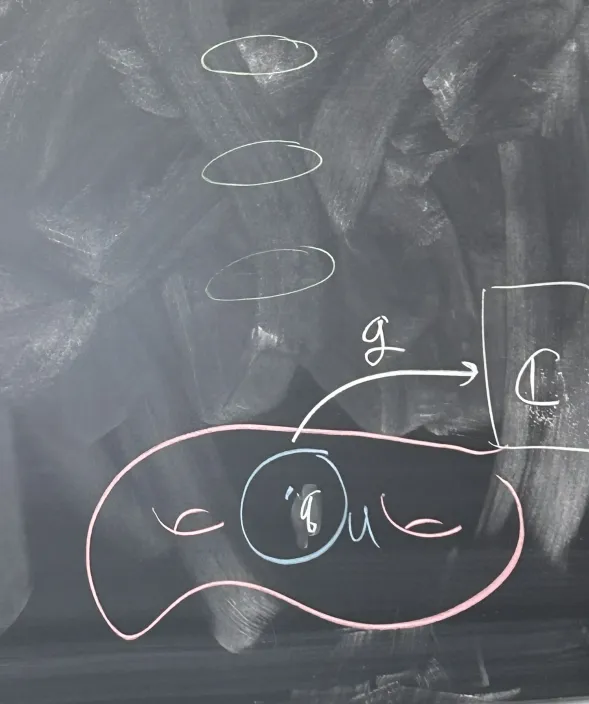
\includegraphics[width=0.5\textwidth]{Figures/lec8-1.png}\]
     We know that $P(T) = \sum_{k = 0}^{d} c_k(x) T^k$ where $c_k(x) \in M(X)$. Hence for $x = q$ is fixed, we can say that $P(q)[T] = \sum_{k = 0}^d c_k(q) T^k$ has coefficients in the complex numbers, ie. $P(q)[T] \in \Cbb[T]$ when $q$ is fixed. Because the discriminant is non-zero, there are $d$ distinct roots in the complex numbers, furthermore the roots move holomorphically with respect to $x$ and do not intersect in small enough $U$ (as long as $\Delta P$ is non-zero).\\

     Finding the functions $g_1, ..., g_d$ amounts to solving $P_2(q, g_i(q)) = 0$, where we define $P_2(q, w) = P(q)(w)$ (set $x = q$ and $T = w$).\\

     So the germs of $g$ such that $P(q, g(q)) = 0$ form a degree $d$ cover over $X \setminus \{z \in X\ |\ P(z)[T] \notin \Cbb[T] \text{ or } \Delta P(z) = 0\}$. We call the set being subtracted $E$.\\

     Note that clearly $E$ is discrete, so we can complete this cover to a degree $d$ branched cover $Y$ of $X$ over $E$. Note that $E$ will not be discrete if $\Delta P$ is identically zero, this is because we are working over a characteristic zero field and irreducible implies separable. Furthermore, now $g$ is a meromorphic function on $Y$ with $P(g) = 0$.
\end{proof}

\begin{question}
    An automorphism of the Riemann surface $X$ induces an automorphism on the field of Meromorphic functions on $X$. Is this process surjective? In other words, does a field automorphism on $M(X)$ come from an automorphism of $X$.
\end{question}

\subsection{The Mittag-Leffler Problem}

The second unit is about classical theorems on (mostly) compact Riemann surfaces (e.g. $X$).\\

To motivate the first discussion of the unit, we will begin with the \textbf{Mittag-Leffler Problem}.

\begin{question}[Mittag-Leffler Problem]
    Let $X$ be a compact Riemann surface, find $f \in M(X)$ with specified ``principal parts".\\
    
    Suppose $\{q_i\}$ is a collection of discrete points on $f \in M(X)$, we can write each $q_i$ with a coordinate chart $q_i \in V_i$ and $\varphi_i: U_i \to \hat{\Cbb}$. Let's suppose without loss that $\varphi_i(q_i) = 0$, then we can write the power series expansion
    \[f|_{U_i} \circ \varphi_i^{-1}(z) = \sum_{k = -m}^\infty c_k z^k \text{ on $V$}.\]
    With some abuse of notation, when the context is clearly, we will just write $f \circ \varphi_i^{-1}$ as ``$f$ in the coordinate $\varphi_i$".
    \[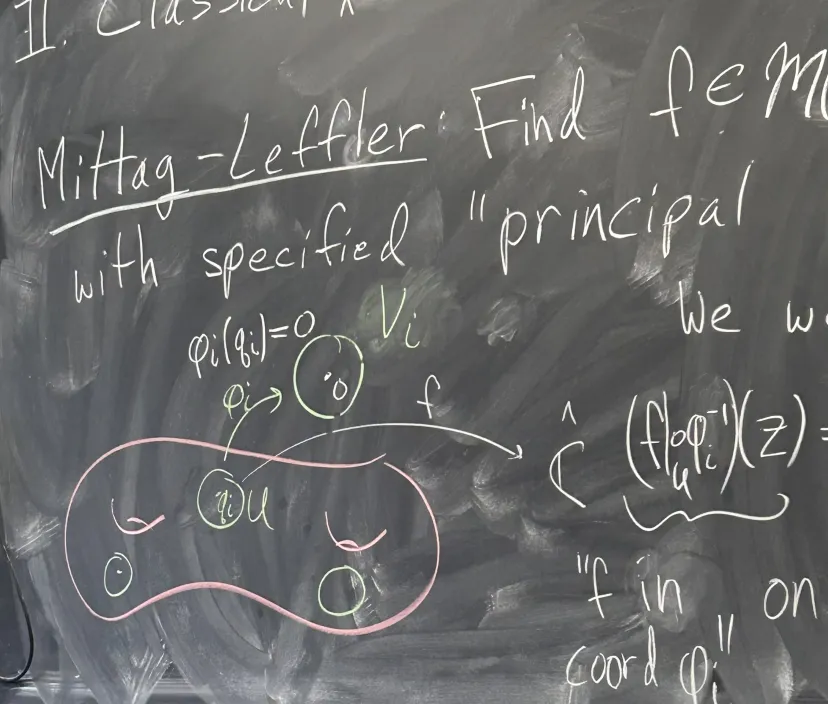
\includegraphics[width=0.5\textwidth]{Figures/lec8-2.png}\]
    In this case, our goal is given $c_{-1}, ..., c_{-m}$ for each $i$, we can construct a meromorphic function $f \in M(X)$ whose $c_{-1}, ..., c_{-m}$ is the specified given values.
\end{question}

Equivalently, this problem may be stated as follows.
\begin{question}
    Given finite set $(U_i, q_i, h_i \in M(U_i)$ such that $h_i|_{U_i - \{q_i\}}$ is holomorphic (it can only have pole on $q_i$). Find $f \in M(X)$ such that $f$ is holomorphic on $X - \{q_i\}_i$ and $f|_{U_i} - h_i$ is holomorphic on $U_i$.
\end{question}

The following proposition shows that the first question can be rephrased in a coordinate-independent way.
\begin{proposition}
    If $f_1, f_2: U_i \to \hat{\Cbb}$ are holomorphic on $U_i \setminus \{q_i\}$, then $f_1 - f_2$ is holomorphic on $U_i$ if and only if $f_1$ and $f_2$ have the same principal part at $q_i$.
\end{proposition}

To solve the Mittag-Leffler Problem, we wish to find $g: X \to \hat{\Cbb}$ such that
\begin{itemize}
    \item $g \equiv h_i$ on some $U_i'$ compactly contained in $U_i$ and $q_i \in U_i'$,.
    \item $g$ is smooth and finite on $X \setminus \{q_i\}$.
    \item In this case, $g$ is a ``weak solution" to the Mittag-Leffler problem.
    \item We want to correct $g$ to a meromorphic function. We do this by adding some function $h$ (with $h$ holomorphic on $U_i'$) to $g$ such that $g + h \in M(X)$.
\end{itemize}

\begin{question}
    How do we find such $h$?
\end{question}

To find $h$, we want it to be a solution to the equation
\[\overline{\partial} h = - \overline{\partial} g\]
on $X$, where $\overline{\partial}$ is to be defined. Then, $\overline{\partial} h  = 0$ on each $U_i' \setminus \{q_i\}$ and $\overline{\partial}(g + h) \equiv 0$ on $X \setminus \{q_i\}$.\\

We want $\overline{\partial}$ to be a differential operator such that 
\[\overline{\partial} f \equiv 0 \text{ on $U$ } \iff f \text{ is holomorphic on } U.\]

\subsection{$\overline{\partial} f$ on the Complex Plane}

Let $U$ be a connected open set in $\Cbb$, and $f \in C^\infty(U)$. We seek to define $\overline{\partial} f \in C^\infty(U)$. Here are some properties, the operator should respect,
\begin{enumerate}
    \item $\overline{\partial}(f(z) + a) = \overline{\partial}(f(z))$, for $a \in \Cbb$.
    \item  $\overline{\partial}(z \mapsto f(z+a)) = z \mapsto \overline{\partial}(f(z + a))$.
    \item  $\overline{\partial}(cf(z)) = c\overline{\partial}(f(z))$.
    \item  $\overline{\partial}(f(z) + g(z)) = \overline{\partial}(f(z)) + \overline{\partial}(g(z))$.
    \item $\overline{\partial}(z \mapsto z) = 0$.
    \item $\overline{\partial}(z \mapsto \overline{z}) = 1$.
    \item $\overline{\partial}(f(z)) = 0$ if $Df(z) = 0$ (all of its first derivatives are zero).
\end{enumerate}

As a consequence of these axioms, we should have that
\[\overline{\partial}(Az + B \overline{z}) = B.\]
We can write any smooth function as
\[f(z) = f(z_0) + A (z - z_0) + B(\overline{z - z_0}) + O(|z - z_0|^2).\]

Using the summation above, if we compute the real partial derivatives, we will get that 
\[\frac{\partial f}{\partial x}(z_0) = A + B.\]
\[\frac{\partial f}{\partial y}(z_0) = i (A - B).\]

We can solve these equations to get
\[A = \frac{1}{2}(\frac{\partial f}{\partial x} - i \frac{\partial f}{\partial y}), B = \frac{1}{2} (\frac{\partial f}{\partial x} + i \frac{\partial f}{\partial y}).\]
In this case, we write that
\[\frac{\partial f}{\partial z} = A \text{ and } \frac{\partial f}{\partial \overline{z}} = B.\]
Sometimes we also write them as $\partial_z f$ and $\partial_{\overline{z}} f$.

Now in this case, $f$ has a complex derivative at $z_0$ if and only if $\frac{\partial f}{\partial \overline{z}}(z_0) = 0$. 

\newpage
\section{Lecture February 29th}

\textbf{Recall:} Last time, we introduced the Mittag-Leffler problem.
\begin{enumerate}
    \item We want to make meromorphic functions on $X$ with specified principal parts.
    \item We can make them by finding ``weak solutions" (meromorphic near specifications and $C^\infty$ else where). Then we can correct the weak solutions by solving the equation $\overline{\partial} h = \alpha$, where $\alpha = \overline{\partial} g$ and $g$ is the weak solution.
    \item For two variable smooth functions on the complex plane, if $f(z) = f(z_0) + A(z - z_0) + B(\overline{z - z_0}) + \mathcal{O}(|z - z_0|^2)$, then we define $\partial_z f \coloneqq A$ and $\partial_z f \coloneqq B$. Then we can derive that
    \[\partial_x f = A + B \text{ and } \partial_y f = i(A - B).\]
    In this case, sooving for $A$ and $B$ gives us that
    \[\partial_z f = A = \frac{1}{2} (\partial_x f - i \partial_y f) \text{ and } \overline{\partial}_z f = B = \frac{1}{2}(\partial_x f + i \partial_y f)\]
\end{enumerate}

\begin{remark}
    In the language of differential forms, we can write
    \[dz \coloneqq dx + idy \text{ and } \overline{dz} = dx - idy.\]
    In this case we have that
    \[d\overline{z} \wedge dz = i dx \wedge dy - i dy \wedge dx = 2i (dx \wedge dy).\]
    Furthermore, this means that as exterior derivatives we can write
    \[df = \partial_x f dx + \partial_y f dy = \partial_z f dz + \partial_{\overline{z}} f \overline{dz}.\]
\end{remark}

\begin{theorem}
    If $U \subseteq \Cbb$ is compact with piecewise $C^1$ boundary $\partial U$, and $f: U \to \Cbb$ is $C^1$, 
    \[\int_{\partial U} f(z) dz = 2i \int_{U} \partial_{\overline{z}} f(z) dx dy, z = x + iy.\]
    Note that the RHS is equal to $\int \partial_{\overline{z}} f(z) d\overline{z} \wedge dz = \int_U df \wedge dz$ (in the language of Differential Forms). In other words, this is simply an application of Stoke's Theorem for differential forms.
\end{theorem}

\begin{proof}
    We will present an elementary proof without using the generalized Stoke's Theorem. We first prove this when $U$ is a rectangle with sides $A, B, C, D$ oriented as
    \[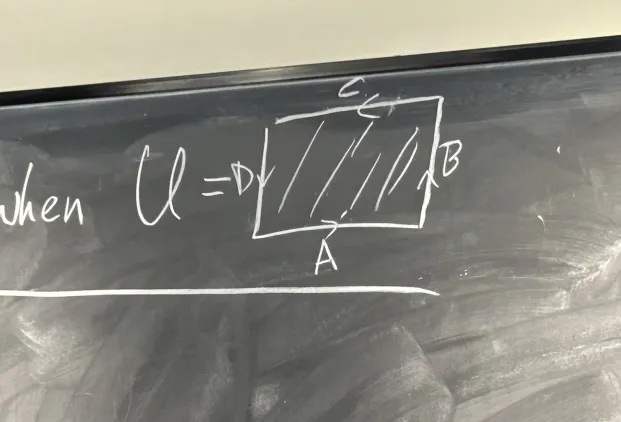
\includegraphics[width=0.5\textwidth]{Figures/lec9-1.png}\]
    Indeed, we can compute the integral to see that
    \begin{align*}
        \int_{U} \partial_{\overline{z}} f dx dy &= \frac{1}{2} \int_{U} \partial_x f dx dy + \frac{i}{2} \int_{U} \partial_y f dx dy\\
        &= \frac{1}{2} \left(\int_B f dy - \int_D f dy \right) + \frac{i}{2} \left( \int_C f dx - \int_A f dx \right) \tag*{Fundamental Theorem of Calculus with respect to one variable}\\
        &= \frac{1}{2} (\int_{B} f \frac{dz}{i} - \int_{D} f \frac{-dz}{i}) + \frac{i}{2} (\int_{C} f(-dz) - \int_{A} f dz) \tag*{Recall $dz = dx + idy$}\\
        &= \frac{1}{2i} \int_{\partial U} f dz.
    \end{align*}
    More a general $U$, we can approximate it by an open set with polygonal boundary, which itself can be approximated by an open set with boundaries composed of vertical and horizontal line segments (which can then be broken down into rectangles).
\end{proof}

\begin{exercise}
        Make the discussion for the general case rigorous.
    \end{exercise}

Recall that for $f: X \to \Cbb$ (or replace $\Cbb$ with any vector space), then
\[\operatorname{supp} f = \operatorname{closure}(\{x \in X\ |\ f(x) \neq 0\}).\]

\begin{definition}
Now suppose $f: \Cbb \to \Cbb$ has compact support, meaning that $\operatorname{supp}(f) \subseteq D_R$ for some $R > 0$. For any $z \in \Cbb$, we define
\[Pf(z) \coloneqq \frac{1}{\pi} \int_{\Cbb} \frac{f(\zeta)}{z - \zeta} d\xi d\eta,\quad \zeta = \xi + i \eta.\]
Is this well-defined? Is this absolutely convergent or are we talking about a principal value? Well, rewriting this in polar coordinates, we write $\zeta = z + r e^{i\theta}$, we have that the integral is
\[Pf(z) \coloneqq \frac{1}{\pi} \int_{0}^{\infty} \int_{0}^{2\pi}  \frac{f(z + re^{i\theta})}{-r e^{i\theta}} r d\theta dr\]
\[= \frac{-1}{\pi} \int_0^\infty \int_0^{2\pi} f(z + r e^{i \theta}) e^{i \theta} dr d\theta.\]
\[= \frac{-1}{\pi} \int_0^{R + |z|} \int_0^{2\pi} f(z + r e^{i \theta}) e^{i \theta} dr d\theta, \quad \text{$f$ has compact support}\]
which implies that the integral is absolutely convergent.
\end{definition}

Hence, $Pf(z)$ is convergent and well-defined. Furthermore, our estimate gives us a proof that
\begin{proposition}
    $|Pf(z)| \leq 2 (R + |z|) ||f||_\infty$. 
\end{proposition}

Similarly, because of the absolute convergence, we will also have that
\begin{proposition}
    Suppose $f$ is $C^{|\alpha|}$, then
    $$D_\alpha Pf(z) = P(D_\alpha f)(z)$$,
    where $D_\alpha = \frac{\partial}{\partial x^k} \frac{\partial}{\partial y^\ell}$ and $|\alpha| \coloneqq k + \ell$.
\end{proposition}

This leads us to the following theorem.
\begin{theorem}
    For $f: \Cbb \to \Cbb$ that is a $C^1$ function with compact support, then
    \[(\partial_{\overline{z}} Pf)(z) = f(z).\]
    Note that this means that $Pf$ is holomorphic outside of the support of $f(z)$.
\end{theorem}

\begin{proof}
    It suffices for us to show that for all rectangles $U$, 
    \[\int_{U} \partial_{\overline{z}} Pf(z) dx dy = \int_{U} f(z) dx dy.\]
    By our version of Green's Theorem derived earlier in this lecture, we have that
    \begin{align*}
        \int_U \partial_{\overline{z}} Pf(z) dx dy &= \frac{1}{2i} \int_{\partial U} Pf(z) dz\\
        &= \frac{1}{2i} \int_{\partial U} \left(\frac{1}{\pi}\int_{D_{R + |z| + 1}} \frac{f(\zeta)}{z - \zeta} d\xi d\eta \right) dz\\
        &= \frac{1}{2i} \int_{D_{R + |z| + 1}} f(\zeta) \left(\frac{1}{\pi}\int_{\partial U} \frac{dz}{z - \zeta}\right) d\xi d\eta \tag*{Fubini-Tonelli Theorem because of absolute convergence}
    \end{align*}
    What is the integral $\int_{\partial U} \frac{dz}{z - \zeta}$? Well it is the winding number of $\partial U$ around $\zeta$ multiplied with $2 \pi i$. Hence we have that
    \[\int_{\partial U} \frac{dz}{z - \zeta} = 2\pi i \mathbbm{1}_{U}(\zeta) = 2\pi i \chi_U(\zeta).\]
    Hence we have that
        \begin{align*}
        \int_U \partial_{\overline{z}} Pf(z) dx dy &= \frac{2\pi i}{2\pi i} \int_{D_{R + |z| + 1}} f(\zeta) \chi_U(\zeta) d\xi d\eta\\
        &= \int_{U} f(\zeta) d\xi d\eta.
    \end{align*}
\end{proof}

\begin{theorem}
    The following are equivalent for $\operatorname{supp}(f) \subseteq D_R$ and $f \in C^1$,
    \begin{enumerate}
        \item $\operatorname{supp}(Pf)$ is compact.
        \item $\operatorname{supp}(Pf) \subseteq D_R$.
        \item $\int_{D_R} fh = 0$ for all holomorphic functions $h: D_R \to \Cbb$.
    \end{enumerate}
\end{theorem}

\begin{proof}
   Clearly (2) implies (1). Now for (1) implies (2), we know that $Pf$ is holomorphic outside of the support of $f$ from the last theorem, hence $Pf$ is holomorphic outside of $D_R$. On the other hand, we know that $Pf \equiv 0$ near $\infty$ because we assumked $\operatorname{supp}(Pf)$ is compact, hence $Pf \equiv 0$ outside of $D_R$ by the identity theorem.\\

   For (3) implies (2), in this case, we have that $Pf(z) = \int_{D_R} \frac{f(\zeta)}{\zeta - z} d\xi d\eta$. We can write the RHS as
   \[Pf(z) = \int_{D_R} f h_z, h_z(\zeta) = \frac{1}{\zeta - z},\]
   and $h_z(\zeta)$ will be a holomorphic function as long as $z \notin D_R$. Hence, by (3), we have that
   \[Pf(z) = 0, \forall z \notin D_R.\]

   For (2) implies (3), we can write
   \[\int_{D_R} fh = \int_{D_{R'}} f h, \text{ for some } R' < R\]
   This is just a technical point to get $h$ continuous on boundary. In this case we have that
   \begin{align*}
       \int_{D_{R'}} fh &= \int_{D_{R'}} (\partial_{\overline{z}} Pf) h\\
       &=  \int_{D_{R'}} \partial_{\overline{z}}( (Pf)h)\tag*{$\partial_{\overline{z}}(gh) = \partial_{\overline{z}}(g) h + g (\partial_{\overline{z}}(h)) = \partial_{\overline{z}}(g) h + 0 $}\\
       &= \int_{\partial D_{R'}} Pf(z) h(z) dz\\
       &= 0 \tag*{Support of $Pf(z)$ is contained in $D_R$.}
   \end{align*}
\end{proof}

\newpage
\section{Lecture March 5th}
Let $U \subseteq \Cbb$ be an open connected set. Let $\mathcal{E}(U) \coloneqq C^\infty(U)$. For any $f \in \mathcal{E}(U)$, we have that
\[D_\alpha f \coloneqq \frac{\partial^{k+\ell}}{\partial x^k \partial y^\ell} f \in \mathcal{E}(U),\]
where $\alpha = (k, \ell) \in \Nbb^2$ is a multi-index and $|\alpha| = k + \ell$.\\

For $m \in \Nbb$ and $K \subseteq U$ compact, we define
\[||f||_{m, K} \coloneqq \sup_{z \in K, |\alpha| \leq m} |D_\alpha f(z)|.\]

We can take a compact exhaustion $K_n$ of $U$ with $K_n \subseteq \operatorname{Int}(K_{n+1})$ and $\bigcup K_n = U$. We can define
\[||f||_{m, n} \coloneqq ||f||_{m, K_n}.\]

We define a topology on $\mathcal{E}(U)$ with the condition that $\lim_{t \to \infty} f_t \to f$ if and only if for all $m, n$, 
\[\lim_{t \to \infty} ||f_t - f||_{m, n} \to 0.\]

\subsection{Topological Vector Space}

\begin{definition}
    A \textbf{topological vector space} $V$ is a vector space over $\Rbb$ or $\Cbb$ (denote the field as $\mathbb{F}$) with a Hausdorff topology $\tau$ on $V$ such that the following maps are continuous:
    \begin{enumerate}
        \item $V \times V \to V$ given by $(x, y) \mapsto x + y$.
        \item $\mathbb{F} \times V \to V$ given by $(\lambda, x) \mapsto \lambda x$.
    \end{enumerate}
\end{definition}

\begin{definition}
    A \textbf{seminorm} on a vector space $V$ is a map $||\bullet||: V \to [0, \infty)$ such that
    \begin{enumerate}
        \item $||f + g|| \leq ||f|| + ||g||$.
        \item $||\lambda f|| = |\lambda| ||f||$.
    \end{enumerate}
    A seminorm is furthermore a norm if additionally $||f|| = 0$ implies that $f = 0$.
\end{definition}

\begin{definition}
Given a collection of seminorms $\{||\bullet||_\alpha\ |\ \alpha \in A\}$ such that if for all $\alpha$, $||f||_\alpha = 0$, then $f = 0$.\\

We can define a \underline{topology} on $V$ generated by the open sets of the form
\[\{B_{\alpha, r}(g) \coloneqq \{f\ |\ ||f - g||_\alpha < r\}, \]
indexed over all $\alpha$ and all $r$.
In this case, $V$ is called a \textbf{locally convex topological vector space}.
\end{definition}

\begin{definition}
    A \textbf{Frechet} space is a locally convex topological vector space from a family of seminorms indexed by $\alpha$. The topology is metrizable, and we can convert this into a metric by
    \[d(f, g) \coloneqq \sum_{\alpha = 1}^\infty 2^{-\alpha} h(||f - g||_\alpha),\]
    where $h(x) = \frac{x}{1 + x}$. We also want to require that this metric is complete.
\end{definition}

\begin{example}
    For $f \in C^0(U)$ (the continuous functions), and $K_n$ is a compact exhaustion of $U$, we can define 
    \[||f||_n \coloneqq \sup_{x \in K_n} |f(x)|.\]
    This is indeed a family of seminorms (they are not norms!) Hence we can give a topology on $C^0(U)$ as a Frechet space. This is also the \textbf{topology of uniform convergence on compact sets (normal convergence)}.
\end{example}

Let $D(U) \coloneqq = \{f \in \mathcal{E}(U)\ |\ \operatorname{supp}(f) \text{ is compact}\}$ (ie. $C^\infty_0(U)$). We also \underline{want a topology} on $D(U)$ such that $f_n \to f$ in $D(U)$ if and only if $f_n \to f$ in $\mathcal{E}(U)$ AND there exists compact $K \subseteq U$ such that for all $n$,
\[\operatorname{supp} f_n \subseteq K.\]

\begin{remark}
   The topology we seek on $D(U)$ is certainly not the subspace topology. 
\end{remark}

\begin{definition}
    The topology we will construct is as follows. For any $h; U \to [0, \infty)$ continuous and $m \in \Nbb$, for any $f \in D(u)$, we let 
    \[||f||_{h, m} \coloneqq \sup_{z \in U, |\alpha| \leq m} h(z) |D_\alpha f(z)|.\]
    These semi-norms define the topology of $D(U)$ as described in the definition earlier. (This is not a Frechet space because the family is not countable).
\end{definition}

\begin{exercise}
    Show that this definition agrees with the topology we wanted to construct.
\end{exercise}

We will also leave the folllowing theorem as an exercise.
\begin{theorem}
    Let $U, V$ be domains in $\Cbb$. If $g: U \to V$ is a diffeomorphism, then $g^*: \mathcal{E}(V) \to \mathcal{E}(U)$ (resp. $g^*: D(V) \to D(U)$) given by
    \[g^* f = f \circ g\]
    is an isomorphism of topological vector spaces.
\end{theorem}

\subsection{Distribution}

\begin{definition}
    A \textbf{distribution} $T \in D(U)^*$ on $U$ is $\Cbb$-valued continuous $\Cbb$-linear functional on $\mathcal{D}(U)$.
\end{definition}

\begin{example}
    If $g \in C^0(U)$, then we can define
    \[\underline{g}: D(U) \to \Cbb\]
    defined by
    \[\underline{g}(f) = \int_{U} fg.\]
    Note that this is well-defined because $f$ is compact support, and this is a distribution.
\end{example}

More generally, if $\mu$ is any locally finite signed Borel measure on $U$ (locally finite means on any compact set it should have finite measure), then the map
\[f \mapsto \int_{U} f d\mu\]
is a distribution.\\

Even more generally, suppose $(\mu_\alpha)_{|\alpha| \leq m}$ is a collection of these kind of measures, then
\[f \mapsto \sum_{\alpha} \int D_\alpha f (d\mu_\alpha) \in D(U)^*.\]

\subsection{Weyl's Lemma}

\begin{theorem}[Holomorphic Weyl's Lemma]
   Let $U \subseteq \Cbb$ be a domain. If $F \in D(U)^*$ is a distribution such that
   \[F(\overline{\partial}g) = 0, \forall g \in D(U),\]
   then there exists $f $ holomorphic on $U$ such that
   \[F = \underline{f}.\]
   In other words, we have that
   \[F(g) = \int_{U} fg, \forall g \in D(u).\]
\end{theorem}

\begin{remark}
    There's also a version of the theorem where $\overline{\partial} g$ is replaced woth $\Delta g$. This is the harmonic version of Weyl's Lemma usually seen in PDEs.
\end{remark}

To prove Weyl's Lemma, we want to make sense of differentiation of distributions (otherwise known as a weak derivative). 
\begin{definition}[Weak Derivative]
    For multindex $\alpha \in \Nbb^2$ and $f \in \mathcal{E}(U)$ and $g \in D(U)$, then
    \begin{align*}
        \int_{U} (D_\alpha f) g \coloneqq (-1)^\alpha \int_{U} f D_\alpha g \tag*{Repeated Integration By Parts}.
    \end{align*}
    This motivates a definition where we define for $T \in D(u)^*$ a distribution as
    \[(D_\alpha T)(g) \coloneqq (-1)^{|\alpha|} T(D_\alpha g).  \]
\end{definition}

\begin{example}
    Let $T \in D^*(U)$ be a distribution. We define $\partial_{\overline{z}} T$ as
    \[\partial_{\overline{z}} T \coloneqq \frac{1}{2} (\partial_x T + i \partial_y T),\]
    where $\partial_x T$ and $\partial_y T$ are defined in the weak sense.\\

    Note that this means that $T(\overline{\partial} g) = \partial_{\overline{z}} T$.
\end{example}


\begin{theorem}
    Suppose $U, V \subseteq \Cbb$ are domains, $g \in D(U \times V)$ (with coordinates $\zeta$ and $z$), and $T \in D(U)^*$, then
    \[D_\alpha(z \mapsto T(\zeta \mapsto g(\zeta, z))\ ) = T(\zeta \mapsto D_\alpha (z \mapsto g(\zeta, z)\ ). \]
\end{theorem}

\begin{proof}
    Exercise.
\end{proof}

\begin{theorem}
    Suppose $U, V \subseteq \Cbb$ are domains, $g \in D(U \times V)$ (with coordinates $\zeta$ and $z$), and $T \in D(U)^*$, then
    \[\int_{U} T(\zeta \mapsto g(\zeta, z)) dx dy = T(\zeta \mapsto \int_{U} g(\zeta, z) dx dy).\]
\end{theorem}

\begin{proof}
    Exercise.
\end{proof}

\end{document}